%%%%%%%%%%%%%%%%%%%%%%%%%%%%%%%%%%%%%%%%%%%%%%%%%%%%%%%%%%%%%%%%%%%%%
%%                                                                 %%
%% Please do not use \input{...} to include other tex files.       %%
%% Submit your LaTeX manuscript as one .tex document.              %%
%%                                                                 %%
%% All additional figures and files should be attached             %%
%% separately and not embedded in the \TeX\ document itself.       %%
%%                                                                 %%
%%%%%%%%%%%%%%%%%%%%%%%%%%%%%%%%%%%%%%%%%%%%%%%%%%%%%%%%%%%%%%%%%%%%%

%%\documentclass[referee,sn-basic]{sn-jnl}% referee option is meant for double line spacing

%%=======================================================%%
%% to print line numbers in the margin use lineno option %%
%%=======================================================%%

%%\documentclass[lineno,sn-basic]{sn-jnl}% Basic Springer Nature Reference Style/Chemistry Reference Style

%%======================================================%%
%% to compile with pdflatex/xelatex use pdflatex option %%
%%======================================================%%

%%\documentclass[pdflatex,sn-basic]{sn-jnl}% Basic Springer Nature Reference Style/Chemistry Reference Style

%%\documentclass[sn-basic]{sn-jnl}% Basic Springer Nature Reference Style/Chemistry Reference Style
\documentclass[bst/sn-mathphys]{sn-jnl}% Math and Physical Sciences Reference Style
\usepackage{subfigure}
\usepackage{multirow}
%%\documentclass[sn-aps]{sn-jnl}% American Physical Society (APS) Reference Style
%%\documentclass[sn-vancouver]{sn-jnl}% Vancouver Reference Style
%%\documentclass[sn-apa]{sn-jnl}% APA Reference Style
%%\documentclass[sn-chicago]{sn-jnl}% Chicago-based Humanities Reference Style
%%\documentclass[sn-standardnature]{sn-jnl}% Standard Nature Portfolio Reference Style
%%\documentclass[default]{sn-jnl}% Default
%%\documentclass[default,iicol]{sn-jnl}% Default with double column layout

%%%% Standard Packages
%%<additional latex packages if required can be included here>
%%%%

%%%%%=============================================================================%%%%
%%%%  Remarks: This template is provided to aid authors with the preparation
%%%%  of original research articles intended for submission to journals published 
%%%%  by Springer Nature. The guidance has been prepared in partnership with 
%%%%  production teams to conform to Springer Nature technical requirements. 
%%%%  Editorial and presentation requirements differ among journal portfolios and 
%%%%  research disciplines. You may find sections in this template are irrelevant 
%%%%  to your work and are empowered to omit any such section if allowed by the 
%%%%  journal you intend to submit to. The submission guidelines and policies 
%%%%  of the journal take precedence. A detailed User Manual is available in the 
%%%%  template package for technical guidance.
%%%%%=============================================================================%%%%

\jyear{2021}%

%% as per the requirement new theorem styles can be included as shown below
\theoremstyle{thmstyleone}%
\newtheorem{theorem}{Theorem}%  meant for continuous numbers
%%\newtheorem{theorem}{Theorem}[section]% meant for sectionwise numbers
%% optional argument [theorem] produces theorem numbering sequence instead of independent numbers for Proposition
\newtheorem{proposition}[theorem]{Proposition}% 
%%\newtheorem{proposition}{Proposition}% to get separate numbers for theorem and proposition etc.

\theoremstyle{thmstyletwo}%
\newtheorem{example}{Example}%
\newtheorem{remark}{Remark}%

\theoremstyle{thmstylethree}%
\newtheorem{definition}{Definition}%

\raggedbottom
%%\unnumbered% uncomment this for unnumbered level heads

\begin{document}
\bibliographystyle{plain}


\title[SmartOPT: A Framework Releasing Compiler Power]{\emph{SmartOPT}: A Framework Releasing Compiler Power}

%%=============================================================%%
%% Prefix	-> \pfx{Dr}
%% GivenName	-> \fnm{Joergen W.}
%% Particle	-> \spfx{van der} -> surname prefix
%% FamilyName	-> \sur{Ploeg}
%% Suffix	-> \sfx{IV}
%% NatureName	-> \tanm{Poet Laureate} -> Title after name
%% Degrees	-> \dgr{MSc, PhD}
%% \author*[1,2]{\pfx{Dr} \fnm{Joergen W.} \spfx{van der} \sur{Ploeg} \sfx{IV} \tanm{Poet Laureate} 
%%                 \dgr{MSc, PhD}}\email{iauthor@gmail.com}
%%=============================================================%%

\author[1]{\fnm{Jinwei} \sur{Zhao}}\email{xxx@gmail.com}

\author[1]{\fnm{Qi} \sur{Zhu}}\email{qizhu\_cs@163.com}
%\equalcont{These authors contributed equally to this work.}

\author[1]{\fnm{Wei} \sur{Wu}}\email{xxx@gmail.com}

\affil[1]{\orgname{Jiangnan Institute of Computing Technology}, \orgaddress{\street{Shanshui Dong Lu}, \city{Wuxi}, \postcode{214000}, \state{Jiangsu}, \country{China}}}

%%==================================%%
%% sample for unstructured abstract %%
%%==================================%%

\abstract{As it is well known to all, performance tuning is a time consuming 
progress. In the modern mainstream compiler, thanks to the coarse-grained 
organization of the optimizing techniques, the performance of programs may be 
improved by just replacing the compiling option level from \emph{-O2} to 
\emph{-O3}. However, this optimizing level strategy ignores 
the details of the underlining architecture and the inherence of the program. 
The opportunities for the further improvement may be 
omitted. To break the constraint of the strategy and to release more power of a 
compiler, we proposed \emph{SmartOPT}. With the help of the static features of 
the source codes and the proposed heuristic predicting model, \emph{SmartOPT} 
makes fine-grained optimizing decisions. A spectrum of evaluations illustrate 
the effectiveness of \emph{SmartOPT}, which can improve the performance of 
programs either based on \emph{-O2} level or \emph{-O3} level. 
Comparing with the 
state-of-art, \emph{SmartOPT} shows great advantage on the overhead of time
with the similar ability to speed programs up. This makes our framework as a 
practicable solution in the engineering field.}

%%================================%%
%% Sample for structured abstract %%
%%================================%%

% \abstract{\textbf{Purpose:} The abstract serves both as a general introduction to the topic and as a brief, non-technical summary of the main results and their implications. The abstract must not include subheadings (unless expressly permitted in the journal's Instructions to Authors), equations or citations. As a guide the abstract should not exceed 200 words. Most journals do not set a hard limit however authors are advised to check the author instructions for the journal they are submitting to.
% 
% \textbf{Methods:} The abstract serves both as a general introduction to the topic and as a brief, non-technical summary of the main results and their implications. The abstract must not include subheadings (unless expressly permitted in the journal's Instructions to Authors), equations or citations. As a guide the abstract should not exceed 200 words. Most journals do not set a hard limit however authors are advised to check the author instructions for the journal they are submitting to.
% 
% \textbf{Results:} The abstract serves both as a general introduction to the topic and as a brief, non-technical summary of the main results and their implications. The abstract must not include subheadings (unless expressly permitted in the journal's Instructions to Authors), equations or citations. As a guide the abstract should not exceed 200 words. Most journals do not set a hard limit however authors are advised to check the author instructions for the journal they are submitting to.
% 
% \textbf{Conclusion:} The abstract serves both as a general introduction to the topic and as a brief, non-technical summary of the main results and their implications. The abstract must not include subheadings (unless expressly permitted in the journal's Instructions to Authors), equations or citations. As a guide the abstract should not exceed 200 words. Most journals do not set a hard limit however authors are advised to check the author instructions for the journal they are submitting to.}

\keywords{Compiling Optimizing, High Performance Computing, Data Analysis}

%%\pacs[JEL Classification]{D8, H51}

%%\pacs[MSC Classification]{35A01, 65L10, 65L12, 65L20, 65L70}

\maketitle

\section{Introduction}\label{sec1}

The human race has entered the Exascale computing era. The complex hierarchy of 
the underlining architecture brings significant performance bonus. Meanwhile, 
programming suffers unprecedented challenge. Programs should be designed in 
a more elegant way to fully utilize the hardwares. Due to the
variety of the \emph{HPC} (High Performance Computing) systems, 
modifications of 
programs or algorithms are neccessary. Code optimizing is never an easy job, 
which usually takes an expert weeks or even months. The complex hierarchy of 
the Exacale computer excerbates the pain. In the Exascale computing era, the 
price we pay for application developing and performance tuning is higher 
than ever. 

Nowadays, more attention has been paied on the parallel models, such as 
\emph{MPI}, \emph{OpenMP}, \emph{CUDA}, \emph{OpenCL}, and so on. 
These models are emerging to alleviate the pain of 
programming on the parallel system. The source code 
transformation on the single core is still important. The performance 
of the source code running on the single core directly affects the performance 
of the entire application. 

Compiler plays an important part on performance. Although tons of compiling 
optimizing techniques have been developed to help people transform source code 
automatically, it is hard to decide which of them should be enabled in certain 
scenarios. In the real world, enabling a compiling optimizing option which is 
supposed to speed up the target source code may incur performance degradation. 
The unexpected impact of the compiling optimizing technique is 
mainly due to the mismatch of the underlining hardware feature and the source 
code transformation. In some cases, the complex interaction among the
optimizing techniques can trigger an unexpected situation. The previous 
optimizing passes may prevent the latter pass being effective. Or 
in a worse case, the interaction degrades the performance. In our previous 
work, we find that by disabling three options (\emph{-fno-tree-vrp}, 
\emph{-fno-tree-sra}, \emph{-fno-tree-ch}) based on \emph{-O3}, the 
manually optimized \emph{GRAPH500} application 
can be speeded up by 27\% in our homemade \emph{HPC} system.

The modern compilers introduce several coarse-grained levels, such as 
\emph{-O0}, \emph{-O1}, \emph{-O2}, \emph{-O3}, \emph{-Os} and \emph{-Ofast}, 
to organize the optimizing techniques. This  
strategy allows people to conventionally utilize the compiler to transform the 
source code for different purposes. It works well in the common cases. However, 
the shortage of this strategy is that it cannot meet the needs of the 
performance sensitive programs. The space 
between the fixed levels is a black box, which is intolerable for the 
\emph{HPC} applications. The specific hardware features and the inherence of 
the source code are ignored. Consequently, the performance 
bonus introduced by the elegant design of the underlining architecture may be 
omitted. In the era of Exascale computing, a compiler should be aware of the 
complex environment to enable the compiling optimizing techniques in the 
fine-grained level accordingly.

Iterative method has been used to evaluate optimizing or parameter setting. It 
profiles the program with different options time and time again to 
find the best options which maximizes the performance. Iterative method 
provides a promissing way to enable the compiling optimizing techniques in the 
find-grained
level. However, the overhead of the iterative progress could be too large to be 
tolerable in the engineering field. Sometimes, it takes hours or even days. 
Besides the iterative method, mathematical model, data mining and machine 
learning have also been studied for years to predict or improve program 
performance based on the profiling data. However, most of them are proven that 
they are only effective on certain type of computing, such as matrix 
multiplication, stencil, vector transformation and so on.

To further release the power of a compiler, we proposed \emph{SmartOPT}, 
a framework 
which breaks the hierarchy of the current optimizing techniques and assists 
people to make fine-grained optimizing decision. \emph{SmartOPT} is composed of 
an offline part and an online part. The offline part is mainly responsible 
for the construction of the pre-trained dataset. Practically, the dataset is 
one of the biggest obstacles to build the predicting model due to the lack of a 
large amount of the source codes to be compiled and evaluated. In our work, a 
random code generator is introduced to fix this. Tons of 
micro-benchmarks are generated to ensure the diversity of the source code 
structure. The static features are extracted from the \emph{AST} 
(Abstract Syntax Tree) to shape the source code in the 
\emph{feature-vector} style. 
Each micro-benchmark is evaluated in the iterative tuning component to get the 
best (local optimal) optimizing options, which are then encoded in the 
\emph{optimizing-vector} style. The \emph{feature-vector} and the 
\emph{optimizing-vector} are 
grouped together to form the basic element of the pre-trained dataset. 

In the online part of \emph{SmartOPT}, the heuristic predicting model is 
designed as a 
replaceable plug-ins. A variant of \emph{KNN} (K-Nearest Neighbour) 
is proposed as the default model. Inspired by the software similarity theory,
the programs are classified into several groups according to the 
\emph{feature-vector}.
The basic heuristic idea is the same source code structure 
(\emph{feature-vector}) can be optimized with the same options 
(\emph{optimizing-vector}). Accuracy 
enhancement is proposed to fix the bias of the predicting model. A spectrum of 
distance weights is introduced in the proposed predicting model to adjust the 
effect of each static feature. The probability based multiple outputs 
mechanism is also introduced. The redundant outputs are necessary due to the 
inaccuracy of the pure static data based predicting model. 

\begin{table}[h]
\begin{center}
\begin{minipage}{\textwidth}
\caption{Comparision of optimizing framework.}\label{TAB1}%
\begin{tabular}{@{}lll@{}}
\toprule
Framework 			& Overhead	& Code structure coverage\\
\midrule
\emph{SmartOPT}    		& Trivial   	& All			\\
\emph{CK}\cite{fursin2021collective}    		& Large		& All	  		\\
\emph{NeuroVectorizer}\cite{haj2020neurovectorizer}	& Trivial	& Loop structure  \\
\emph{FlexTensor}\cite{zheng2020flextensor}	& Trivial	& Tensor computations \\
\emph{DeepTune}\cite{cummins2017end}		& Trivial	& Loop structure \\
\botrule
\end{tabular}
\end{minipage}
\end{center}
\end{table}

As shown in Table~\ref{TAB1}, comparing with the state-of-art, \emph{SmartOPT}
outperforms in two folds. First, as only static features are considered, 
the predicting overhead of \emph{SmartOPT} is trivial (the cost is about 
several seconds), which makes \emph{SmartOPT} more practicable 
than the iterative based frameworks. Second, \emph{SmartOPT} handles the 
common pieces of code, while most of the current mathematical based frameworks 
cover only certain code structures individually. 

Briefly speaking, there are four main contributions.

\begin{enumerate}[1.]
	\item We proposed \emph{SmartOPT}, which provides a way to generate 
	fine-grained compiling optimizing options automatically, further 
	releases the power of a compiler system on performance.

	\item We proposed a novel random code based dataset construction 
	procedure for the compiling evaluation. The rapid construction of 
	dataset introduces a wider scope for applying data analysis 
	techniques in the compiler field.

	\item We proposed a variant of \emph{KNN} model to make prediction
	based on the pure static data with the accuracy enhancement to fix the 
	bias. The overhead and the accuracy of the predicting model achieve a 
	delicate balance.

	\item A comprehensive evaluation reveals the relationship between the 
	configurations of the heuristic predicting model and the predicting 
	accuracy. A promising way is provided for the improvement of 
	\emph{SmartOPT}.
\end{enumerate}

The paper is organized as follows. Section~\ref{sec2} introduces related works.
The overall structure of \emph{SmartOPT} is illustrated in Section~\ref{sec3}. 
In Section~\ref{sec4} and Section~\ref{sec5}, we describe the details of 
\emph{SmartOPT}. Evaluation is provided in Section~\ref{sec6} and 
Section~\ref{sec7} concludes the paper.


\section{Related Work}\label{sec2}

In the last decades, compiling optimizing has attracted the interest of many 
research groups. Tons of technologies have been proposed. But, how to enable 
them efficiently is still an open question. Several methods have been 
introduced to face this challenge.

Iterative compiling is used to probe the combinations of the compiling 
optimizing options. Several 
works~\cite{guo2010auto,nukada2009auto,song2014designing} focus on autotuning
parameters of FFT, SpMV to obtain performance bonus. Concentrating on 
scalar, loop-nest, loop-unroll, polyhedral and other optimizing 
methods~\cite{ashouri2012design,fang2015practical,fursin2002evaluating,
kisuki2000iterative,kisuki2000combined,pouchet2007iterative}, 
fabulous wok has been done by the other research groups. Besides those, a 
notable work is TVM~\cite{chen2018tvm}, which is an automated optimizing 
compiler for deep learning. TVM solves optimization challenges specific to 
deep learning by employing a cost modeling method for rapid exploration of 
code optimizations. Jason et. al. proposed PetaBricks~\cite{ansel2009petabricks}
to autotune programs by making both fine-grained code optimizing as well as 
algorithmic choices, including data distributions, algorithmic parameters, 
transformations, and blocking. Originated from the MILEPOST GCC 
project~\cite{fursin2011milepost}, Collective Knowledge (CK) 
framework~\cite{fursin2021collective} provides a practical engineering solution 
to compile and execute a program in an iterative way. Besides the systematic 
supports for the R\&D community, the iterative progress provides a method to 
evaluate compiler options automatically.

Due to the huge overhead of iterative compiling, some methods have been propose
to reduce the time consumption of iterative progress. 
S.Triantafyllis et. al. proposed a heuristic algorithm to remove the redundant 
optimizing~\cite{triantafyllis2003compiler}. And based on the feedback 
information, the optimizing space is pruned further. The group lead by Keith D. 
Cooper~\cite{chabbi2011efficiently} revealed that genetic algorithm can 
dramatically reduce the size of solution space. In the VISTA framework, Wankang Zhao et. al.~\cite{zhao2002vista}  reduced the iterative overhead by removing 
redundant, useless optimizing with the support of genetic algorithm.

Recent years, based on the pre-trained dataset, data mining and machine 
learning are used to analyse programs. In this field, programs should 
be represented as a list of quantifiable features. 
Several works have been done to extract program features, both static 
features~\cite{fursin2011milepost,ferrante1987program,allen1970control,
park2012using} and dynamic features~\cite{mahlke1992effective,
cavazos2007rapidly,luk2005pin,hoste2007microarchitecture}. Dimension reduction 
of the feature space is also studied with the support of Principle Component 
Analysis and Exploratory Factor Analysis. With the effective feature list, 
supervised learning~\cite{ashouri2016cobayn,ding2015autotuning,
cosenza2017stencil}, such as Bayesian net, decision tree, linear models, and 
unsupervised learning~\cite{martins2014exploration,kulkarni2012mitigating}, 
such as clustering, evolutionary algorithms, are introduced to handle the 
dataset. Different from the iterative methods, machine learning suffers from 
much less predicting overhead. The time consumption is transferred to the 
training progress. The challenge is the predicting 
accuracy, which is influenced by program features, size of dataset, predicting 
model and so on.


\section{Overall structure of \emph{SmartOPT}}\label{sec3}

The motivation that we proposed \emph{SmartOPT} is to maximize the effect of 
the existing compiling optimizing techniques. \emph{SmartOPT} is designed as a 
peripheral supplementary of a compiler system. Cooperating with 
the basic compiling progress, it introduces several novel mechanisms to make 
the find-grained optimizing options decision. 

The overall structure of 
\emph{SmartOPT} is shown in Figure~\ref{FIG1}. It consists of two parts, the 
offline part and the online part. The offline part builds the dataset with the 
help of the random code generator, the iterative tuning component and the 
customized compiler system. Based on the dataset, the online part yields the 
optimizing options according to the structure of the source code. The 
customized compiler system provides the static feature extraction support for 
both parts.

\begin{figure}[h]%
\centering
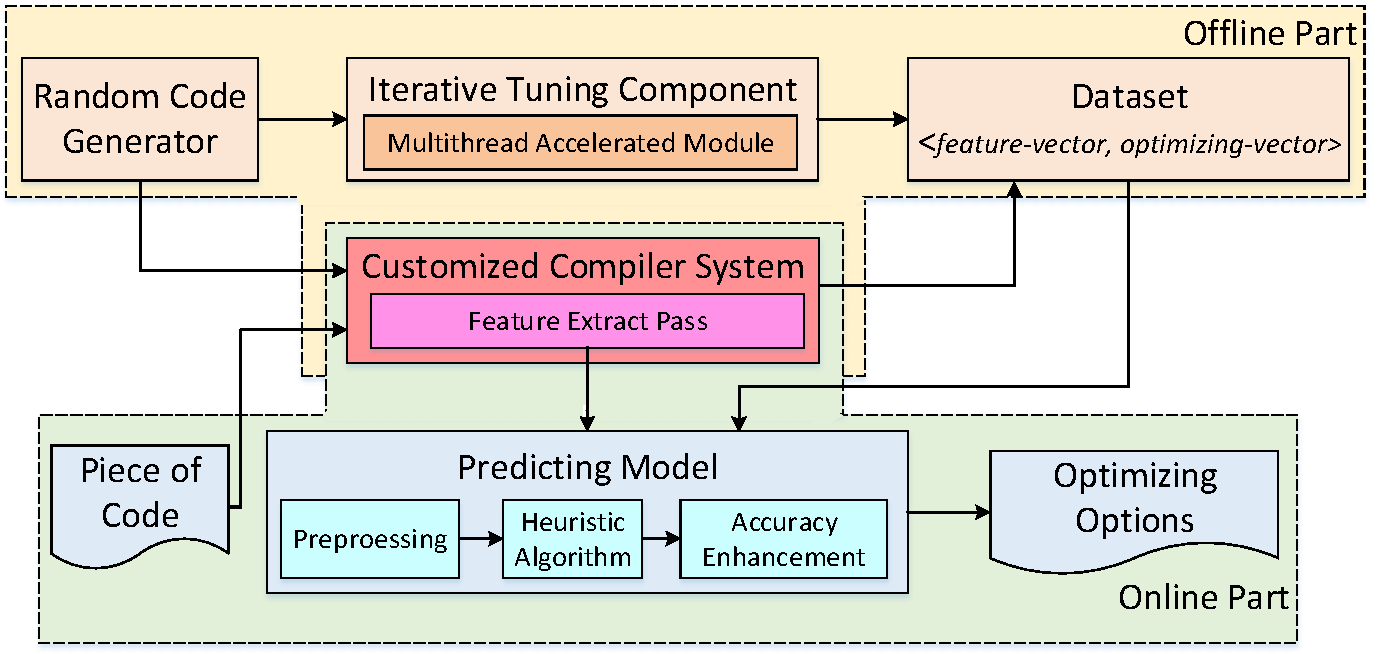
\includegraphics[width=0.7\textwidth]{fig/fig1.pdf}
\caption{Overall structure of \emph{SmartOPT}}\label{FIG1}
\end{figure}


\subsection{The workflow of \emph{SmartOPT}}\label{subsec0301}

Specifically, in the offline part, a novel random code based rapid dataset 
construction procedure is proposed. There are three steps. First, the random 
code generator produces a batch of random code pieces. The diversity of the 
source code structure, which is crucial for the heuristic predicting model, is 
ensured at this step. Second, the iterative tuning component and the customized
compiler system process the random source code one by one, and yield a set of 
static features and a set of optimizing options for each piece of code. 
Finally, the output of the second step is formalized into the style of 
\emph{feature-vector} and \emph{optimizing-vector}. These vectors are grouped 
as a basic element of the dataset and stored in the customized database.

In the online part, a piece of source code is taken as the input. In the 
customized compiler system, the input source code is processed by the feature 
extract pass to generate the \emph{feature-vector}. Then, the 
\emph{feature-vector} is imported into the heuristic predicting model to make 
prediction based on the dataset. A group of optimizing options is yielded as 
the final output of \emph{SmartOPT}. The heuristic predicting model is the key 
of the online part. Three components, preprocessing, heuristic algorithm, 
accuracy enhancement, are introduced to make a tradeoff between the predicting 
accuracy and the predicting speed.

The details of the workflow are described in Section~\ref{sec4} (the offline part) and Section~\ref{sec5} (the online part).

\subsection{The characteristics of \emph{SmartOPT}}\label{subsec0302}

\emph{SmartOPT} is designed as a flexible, portable, agile and quality-cost 
balanced framework. The systematic advantages make \emph{SmartOPT} not only a 
valuable try on academic but also a practical solution in the engineering 
field.

To ensure the flexibility, a modular based component management is introduced. 
The main components of \emph{SmartOPT} are managed as plug-ins. The random 
code generator, the iterative tuning component, the predicting model are 
highly independent with each other. People may replace the current 
implementation with a better one to improve the performance of the entire 
framework. A global description file is used to indicate which implementation 
is enabled for each component. The dataset is generated as needed for the 
specified environment and the customized configurations. 

The implementation of \emph{SmartOPT} is independent with the details of the 
underlining architecture. The hardware and software environments of the target 
computer system are described in the global file. \emph{SmartOPT} can be 
deployed in any computer system with minor changes of the global file, 
showing its great advantage on portability.

The agility of \emph{SmartOPT} is guaranteed in the rapid dataset construction. 
The dataset construction is annoying as the environment is usually variable. 
Any modification of the underling architecture should play a part in the 
dataset so that the bias introduced by the static feature based dataset could 
be minimized. For the concern on the agility of deployment, in \emph{SmartOPT},
the procedure of dataset construction is normalized and automated, supporting 
one-click construction. 

Only static features are used as the input of the predicting model in 
\emph{SmartOPT}. This reduces the overhead of the predicting progress, 
allowing \emph{SmartOPT} to generate result in several seconds. However, due 
to the limited information of the static features, \emph{SmartOPT} suffers the 
problem of inaccurate prediction. In view of this, a spectrum of enhancement 
methods are introduced to achieve the delicate quality-cost balance in 
\emph{SmartOPT}.

\section{Rapid dataset constrution}\label{sec4}

In this section, we describe the details of the rapid dataset construction. 
Random code generator, iterative tuning component and customized compiler 
system are the three main parts. The structure of the dataset element is also 
revealed in this section.

\subsection{Random code generator}\label{sec0401}

% In \emph{SmartOPT}, the random code generator is built based on 
% \emph{CSmith}~\cite{yang2011finding}, which generates random C programs that 
% statically and dynamically conform to the C99 standard. \emph{CSmith} is 
% useful for stress-testing compilers, statics analyzers and other tools. In 
% our 
% work, several modifications are performed, so that the random code generator 
% of \emph{SmartOPT} can yield evaluable random C program for the code 
% structure 
% coverage.

In \emph{SmartOPT}, a random code generator is introduced to yield huge amount 
of micro-benchmarks to meet the needs of code structure diversity.

First, a persistent main function is introduced as the interface of the random 
generated based program. As shown in Figure~\ref{FIG2}, main.c is compiled 
once to generate the object file main.o. In main.c, the statement 
\emph{foo()} marked as red includes the symbol used to invoke the function 
which is composed of the random generated code. To alleviate the impact of the 
runtime system noise, a loop structure is inserted to enclose \emph{foo()}. In 
the default setting, the inserted \emph{for-loop} statements are executed 1000 
times. A couple of 
the timing statements, \emph{timer\_start()} and \emph{timer\_end()}, are 
introduced to record the executing time of \emph{foo()}. 
% It provides a way to 
% evaluate how well the current compiling optimizing options perform in the 
% iterative progress.

\begin{figure}[h]%
\centering
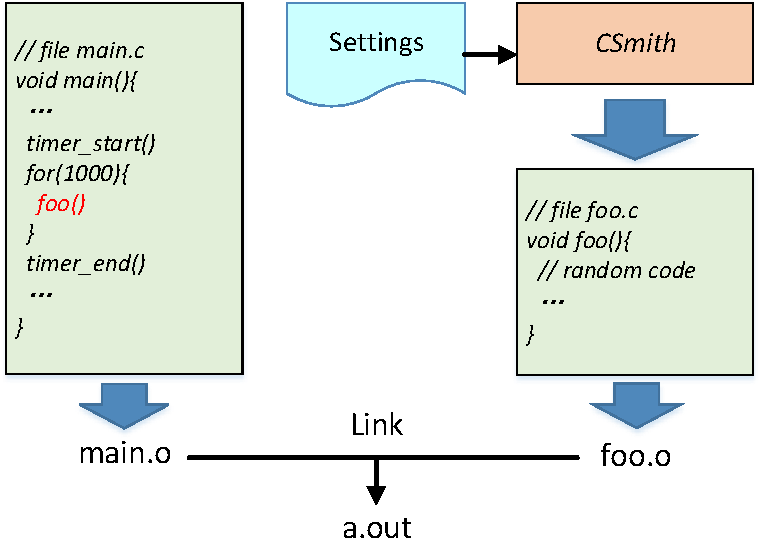
\includegraphics[width=0.5\textwidth]{fig/fig2.pdf}
\caption{The code structure of the random generated program.}\label{FIG2}
\end{figure}

The file foo.c is generated by the random code generator.  
All kinds of C99 language elements, such as data type (e.g. int, long, 
float, double and so on), data array, pointer, if-else-then, for-loop, 
while-loop and so on, are supported in the random code generator. In our 
scenario, only code structure is concerned. For simplicity without losing 
generality, any function call is 
forbidden in the body of \emph{foo()}. The object foo.o is updated for each 
recent generated foo.c.

Finally, main.o and foo.o are linked together to form the executable file a.out 
for the further evaluation.

\subsection{Iterative tuning component}\label{sec0402}

In the iterative tuning component, the random generated program is evaluated 
with different optimizing options iteratively. During this progress, the 
optimizing options which bring the best performance bonus are obtained. These 
optimizing options are taken as a part of the basic element in the dataset 
after being normalized in the style of \emph{optimizing-vector}.

Given the huge overhead of the existing iterative tuning method, we parallelize 
the iterative progress. The iterations are independent with each other. 
Accordingly, we map each iteration to one single thread, which is executed on 
individual CPU core. The results of all threads are reduced after 
synchronization. A validation phase is performed to remove the redundant the 
options which are not effective for the program. The validation step is also 
parallelized. The multithread accelerated iterative module is illustrated in 
Figure~\ref{FIG3}. More details are described in~\cite{jinwei2021}.

\begin{figure}[h]%
\centering
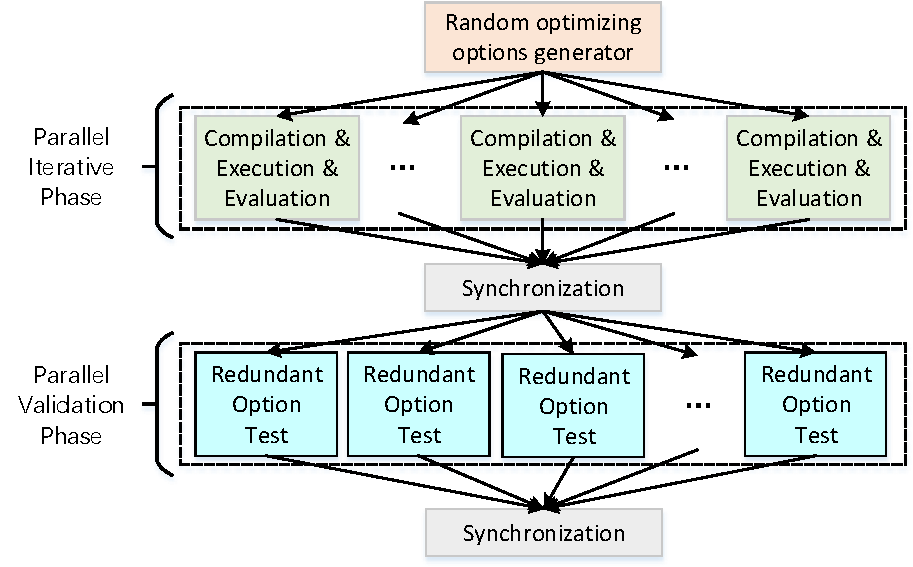
\includegraphics[width=0.5\textwidth]{fig/fig3.pdf}
\caption{The sketch of the mutithread accelerated iterative module.}\label{FIG3}
\end{figure}

\subsection{Customized compiler system}\label{sec0403}

The static features of the source code are extracted in the customized 
compiler system. Among the existing compiling passes of the compiler, a 
customized feature extract pass is inserted for the source code analysis. As 
soon as the \emph{AST} is built, the feature extract pass is performed.

There are two steps for the feature extraction. First, the feature extract 
pass traverses all the paths of the \emph{AST}. The basic elements, such as 
the number of statements, the number of edges, the type of data, the type of 
statement, the arguments of the call statement, the express of rhs and lhs, 
and so on, are captured in the formalized structures. Then, based on these 
structures, the second level extraction is performed to get some meaningful 
features. For example, the number of basic blocks with a single successor, the 
number of basic blocks with two successors, the number of basic blocks in 
loops, the number of critical edges, the average of number of instructions in 
basic blocks, the number of switch instructions in certain methods, the number 
of logical operations in certain methods, and so on, are collected. The second 
level extraction is scalable. People can customize the static features they 
care by modifying the configuration files. Inspired by the previous 
works~\cite{fursin2021collective,fursin2011milepost}, in the default setting, 
\emph{SmartOPT} supports 65 features, covering the type of CFG, instructions, 
phi-nodes, constants, variables and loops.

\subsection{Data structure description}\label{sec0404}

The dataset is organized as a group of basic elements, which can be represented 
as the couple of \emph{feature-vector} and \emph{optimizing-vector}.

The \emph{feature-vector} is composed of the value of static features. It is a 
vector of floating point data. The name of the static feature is omitted in 
the vector as the sequential of these features is fixed. The 
\emph{feature-vector} is taken as the index of the dataset.

To save the memory space occupied by the dataset, the \emph{optimizing-vector} 
is stored in the binary style. The sequence of all the optimizing options of 
the compiler has been orchestrated beforehand. One bit is introduced to 
represent the status of a single option. If the option is enabled, the 
corresponding bit will be set as 1, otherwise, the bit will be set as 0.

The examples of the encoding progress and the decoding progress are illustrated in Figure~\ref{FIG4}. In the encoding progress 1, 
-freorder-blocks-and-partition, -fno-tree-dominator-opts, -funroll-loops, are 
encoded in the optimizing-vector style, which is represented as 
<0 0 0 0 0 0 1024 0 0 32 0 1024 0>. The encoding progress 2 reveals the 
individual bit for each option. The decoding progress translates the 
\emph{optimizing-vector} into the readable options. In \emph{SmartOPT}, the 
scripts encoding\_flags.py and decoding\_flags.py are responsible for the 
encoding progress and the decoding progress.

\begin{figure}[h]%
\centering
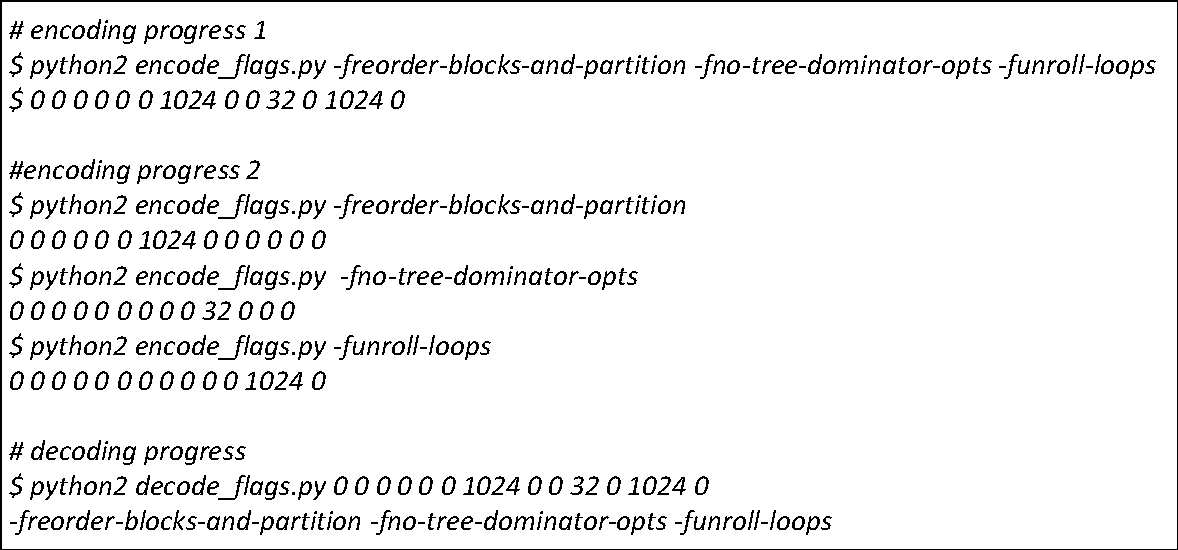
\includegraphics[width=0.6\textwidth]{fig/fig4.pdf}
\caption{The examples of the encoding progress of the \emph{optimizing-vector} 
and the decoding progress of the \emph{optimizing-vector}.}\label{FIG4}
\end{figure}

\section{Heuristic predicting model}\label{sec5}

In \emph{SmartOPT}, the online part makes prediction based on a heuristic 
model. As shown in Figure~\ref{FIG1}, it takes the dataset and the 
\emph{feature-vector} of the target code as input, and yields the 
\emph{optimizing-vector} as output. Preprocessing, heuristic algorithm and 
accuracy enhancement are the three main parts.

\subsection{Preprocessing}\label{sec0501}

Before imported into the heuristic algorithm, the \emph{feature-vector} should 
be formalized so that it can be processed in an effective way.

Firstly, all elements in the \emph{feature-vector} are divided by the number 
of instructions to eliminate the impact of the source code size. Then, 
normalization is introduced to balance the influence of the different elements 
in the vector. The maximum value and the minimum value of each element are 
recorded as the dataset expanded. And each data is divided by the gap between 
of them. Accordingly, the value of the element in the vector is transformed in 
the range of [0, 1].

As the \emph{feature-vector} is extracted from the static \emph{AST}, no 
runtime system noise is introduced. The outlier detection and elimination are 
omitted in the preprocessing.

\subsection{Heuristic algorithm --- A variant of KNN}\label{sec0502}

In the offline part, thanks to the random code generator and the customized 
compiler system, a batch of the pre-trained data is collected, in the form of 
\emph{<optimizing-vector, feature-vector>}. The \emph{feature-vector} 
represents the multi-dimensional coordinates of data in the solution space, 
while the \emph{optimizing-vector} is taken as the tag. For a certain piece of 
code, \emph{SmartOPT} makes the prediction of the \emph{optimizing-vector} 
based on the existing set of the \emph{feature-vector} in the solution space.

We proposed a variant of \emph{KNN} as the heuristic algorithm, which 
transforms the prediction problem to a neighbor probing game. The typical 
\emph{KNN} algorithm makes prediction based on the tags of the K nearest 
neighbors. The most probed tag of these neighbors is the final predicting 
result. As shown in Figure~\ref{FIG5} (a), for the black node, 5 out of 9 
neighbors are marked as \emph{Tag4}, and the other 4 neighbors are marked as 
\emph{Tag2}. So, the prediction for the black node is \emph{Tag4}.

\begin{figure}[h]%
\centering
\subfigure[The typical \emph{KNN}.]{
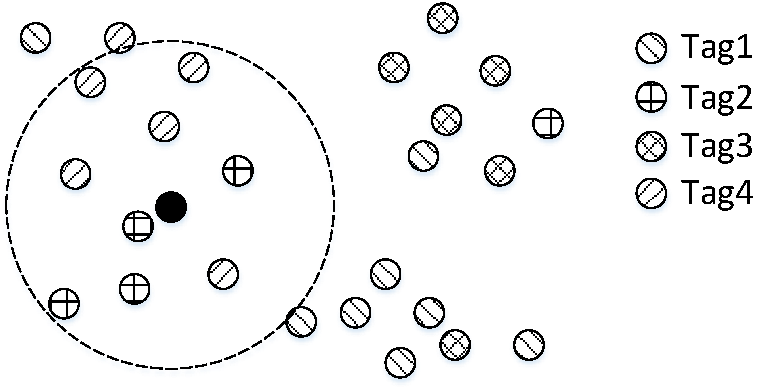
\includegraphics[width=0.4\textwidth]{fig/fig5a.pdf}
}
\subfigure[The proposed variant of \emph{KNN}.]{
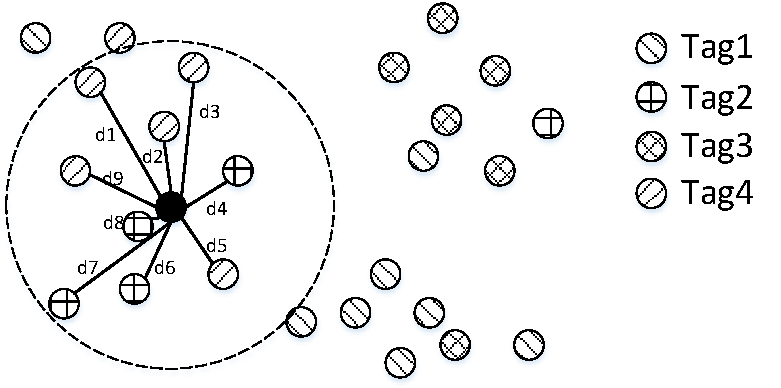
\includegraphics[width=0.4\textwidth]{fig/fig5b.pdf}
}
\caption{The diagram of \emph{KNN} algorithms.}\label{FIG5}
\end{figure}

The shortage of the typical \emph{KNN} is that only the number of neighbors is 
considered. The limited information makes the prediction bias to the most 
probed tags. The more the tags are probed, the more likely they will be 
yielded. In the case that the target node is the same as an existing neighbor, 
if the tag of the neighbor does not have the amount advantage, the output may 
not be the anticipative tag of the neighbor.

To alleviate this bias, in the proposed variant of \emph{KNN}, distance 
between nodes is considered in the heuristic algorithm. As shown in 
Figure~\ref{FIG5} (b), the black node is closed to a neighbor marked as 
\emph{Tag2}, and the distance, \emph{d8}, is much shorter than the others. 
Intuitively, the black node should be more likely marked as \emph{Tag2} due to 
the \emph{feature-vector} similarity. To embody this likelihood, we add the 
distance as an additional metric in the typical \emph{KNN} algorithm. The 
details of the heuristic algorithm are shown in Algorithm~\ref{ALGO1}. 

\renewcommand{\algorithmicrequire}{\textbf{Input:}}
\renewcommand{\algorithmicensure}{\textbf{Output:}}

\begin{algorithm}
\caption{The distance based \emph{KNN} variant.}\label{ALGO1}
\begin{algorithmic}[1]
\Require
The training data set <\emph{optimizing-vector}, \emph{feature-vector}> is 
represented as \emph{D}. The \emph{feature-vector} of the target source code 
is represented as \emph{t}. The threshold of the neighbor number is 
represented as \emph{K}. The distance weight set is represented as \emph{W}.
\Ensure 
The \emph{optimizing-vector} of the target source code.
\For {$d$ in $D$}
\State Compute distance between $d$ and $t$
\State Multiply the computed distance with $W$
\label{s03}
\State Store the result of step~\ref{s03} in $DIS[d]$
\EndFor
\State Reorder $DIS[d]$ in the ascending way
\For {$k$ in the first $K$ elements of $DIS[d]$}
\State Classify the elements based on \emph{optimizing-vector}
\State The classification is represented as $TAG[p]$($p$ <= $k$)
\State Accumulate the $1/DIS[k]$ for $TAG[p]$
\EndFor
\State Reorder $TAG[p]$ in the descending way
\State
\Return The \emph{optimizing-vector} of $TAG[0]$
\end{algorithmic}
\end{algorithm}

\subsection{Accuracy enhancement}\label{sec0503}

To enhance the accuracy of predicting, we also introduce a spectrum of 
distance weights (represented as $W$ in Algorithm~\ref{ALGO1}) in the 
heuristic algorithm. These weights indicate the impact of each element of 
\emph{feature-vector} quantitatively, revealing how easily the corresponding 
feature will be changed if the source code is transformed.

The distance weights in the heuristic algorithm are determined in the 
following way. A set of random micro-benchmarks are collected as the input of 
the feature extract pass. The static features are extracted twice, from the 
original \emph{AST} first, and then from the transformed \emph{AST}. The 
variation of the static features is illustrated in Figure~\ref{FIG6}. The 
darker the node is, the larger the variation is. The average value is 
introduced to quantify the variation. To normalize the difference between 
features, Equation~\ref{EQ2} is used to compute the distance weights. $W$ 
represents 
the distance weight, and the average value of feature difference is represented 
as $V$. $V$ is calculated as shown in Equation~\ref{EQ1}, in which $V1$ 
represents 
the value of the feature extracted in the first time and $V2$ represents the 
value of the feature extracted in the second time.

\begin{figure}[h]%
\centering
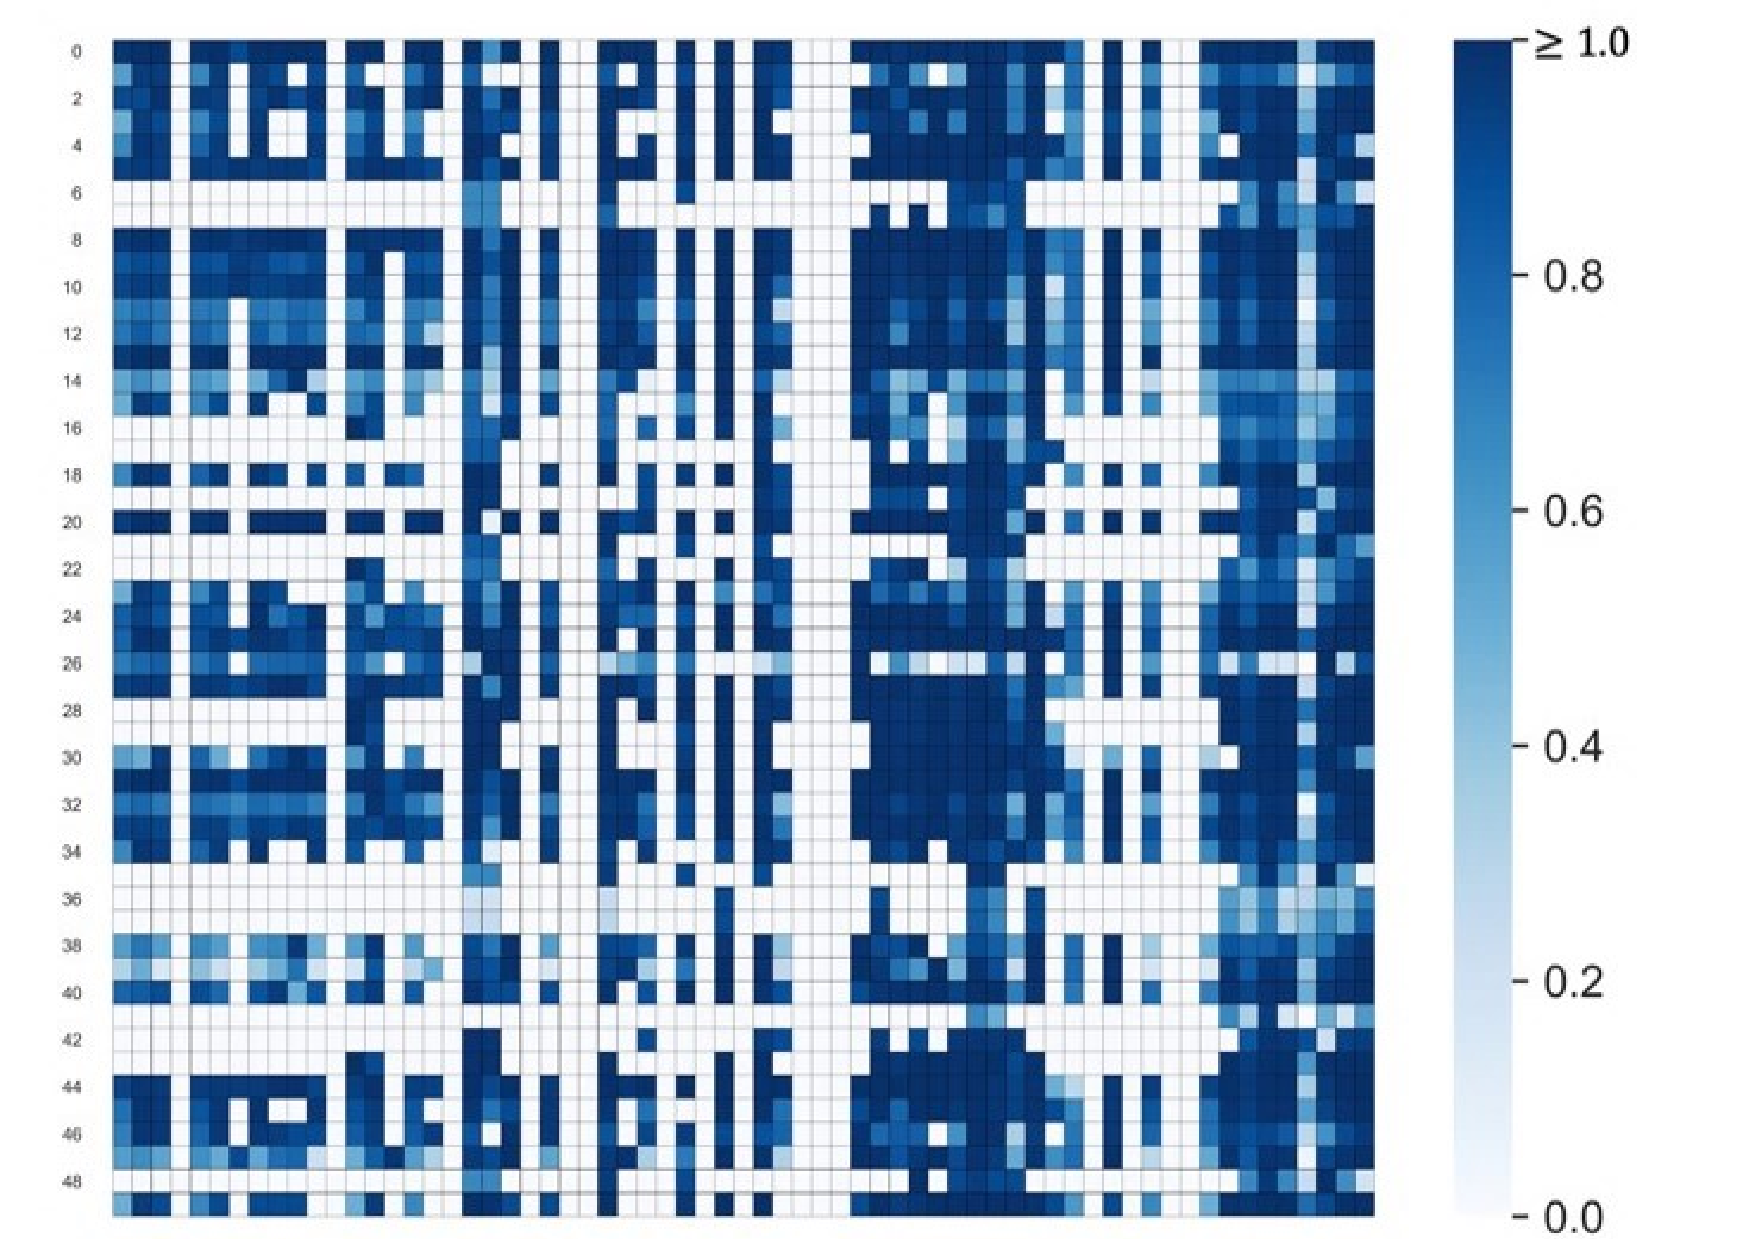
\includegraphics[width=0.6\textwidth]{fig/fig6.pdf}
\caption{The variation of the static features with optimizing with 100 
micro-benchmarks.}\label{FIG6}
\end{figure}

\begin{equation}
	V=\frac{abs(V1-V2)}{V1} \label{EQ1}
\end{equation}


\begin{equation}
W=\left\{\begin{matrix}
10^{(V-0.5)/0.1},&if&10^{(V-0.5)/0.1} < 1 \\
1,&if&10^{(V-0.5)/0.1}\geqslant 1
\end{matrix}\right. \label{EQ2}
\end{equation}

\emph{SmartOPT} predicts optimizing options totally based on the static 
features of the source code. As the predicting accuracy of these static 
analysis methods is the heel of Achilles, we proposed another accuracy 
enhancement in \emph{SmartOPT}. As shown in Algorithm~\ref{ALGO1}, only the 
\emph{optimizing-vector} of $TAG[0]$ is yielded as the output. More outputs 
are likely to cover the other possible optimizing directions to speed up the 
target source code. Inspired by that, we provide a configuration $N$ to support 
multiple outputs for the predicting model. In Section~\ref{sec6}, the 
evaluation is carried out to see how many outputs should be yielded.


\section{Evaluation}\label{sec6}

In this section, \emph{SmartOPT} is evaluated systematically. We first reveal 
the impact of the customizing configurations of the heuristic algorithm, such 
as the size of dataset, the number of neighbors, and the number of outputs. 
Then, with the best configurations obtained, \emph{SmartOPT} is tested based 
on the \emph{SPEC2000} and \emph{SPEC2006} benchmark suites to show the 
effectiveness.

How to evaluate the accuracy of the predicting model is a problem. The 
predicting accuracy is defined as follows in our work. First, a group of 
programs are processed in an iterative way to see whether there is a 
fine-grained optimizing solution to speed up the target program. The amount of 
the speeded up programs is recorded. Then, these programs are exported to the 
predicting model. If the result of the predicting model can improve the 
performance of the program, we will claim that the predicting is accurate. The 
accuracy is the ratio of the number of the predicting solutions to the number 
of the iterative solutions.

The distance involved in the heuristic algorithm is Euler distance. The evaluation is performed on the \emph{SHENWEI TaihuLight} system.

\subsection{Impact of the customizing configurations}

In \emph{SmartOPT}, the number of neighbors and the number of outputs are two 
parameters of the proposed predicting model, which could be configured by 
programmers. To reveal the influence of these parameters, we provide a 
spectrum of tests with the setting of neighbor amount varying from 20 to 100 
and the setting of output amount varying from 1 to 10. The size of dataset is 
also configured as 1000, 2000, 3000 and 4000 individually.

As shown in Figure~\ref{FIG7} (a), when the number of the output is set as 1, the 
predicting accuracy is less than 0.6. The static feature based idea affects the 
predicting accuracy in many ways. First, different from the dynamic features, 
static features only describe the code structure, and they cannot obtain the 
runtime information, incurring interference in the prediction model. Second, 
the introduced interference makes the relationship between predicting accuracy 
and the parameters confusing, which cannot indicate any clue on how to make 
improvement.

To overcome the shortage of the static feature based predicting, we increase 
the amount of the output of the prediction model. As shown in 
Figure~\ref{FIG8}, with multiple settings of the amount of neighbors, the 
predicting accuracy increases as the amount of output increasing. When the 
amount of output is set as 10, the predicting accuracy reaches as high as 
about 0.9, which is a significant improvement compared with 0.6. Furthermore, 
the predicting accuracy curve becomes less steep when the amount of output is 
larger than 8. In the following part, we set the amount of output as 10.

In Figure~\ref{FIG7} (b), we reveal the influence of the amount of neighbors and 
the size of dataset. Across all settings of dataset, the predicting accuracy 
shows an increasing trend when the amount of neighbor increases. In the 100 
neighbor case, the predicting accuracy of 3 out of 4 bars reaches 0.89. The 
1000 dataset shows a small drawback (about 0.03) on accuracy. In general, the 
trend of predicting accuracy increases when the size of dataset increases. Two 
exceptions (20 neighbors and 60 neighbors) are illustrated in the 1000 dataset 
case, which is due to the predicting biased introduced by the limited size of 
dataset.


\begin{figure}[h]%
\centering
\subfigure[The typical \emph{KNN}.]{
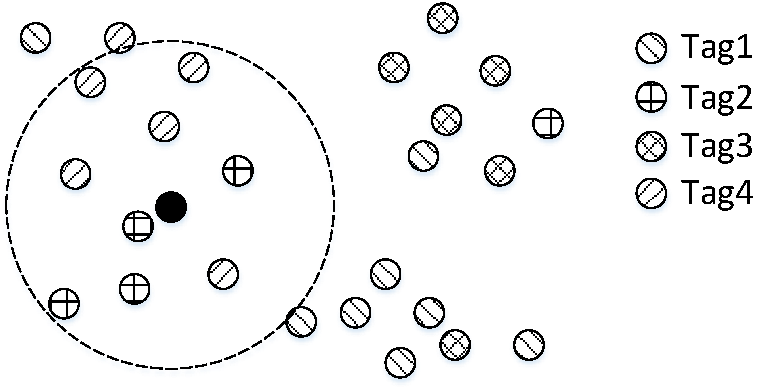
\includegraphics[width=0.4\textwidth]{fig/fig5a.pdf}
}
\subfigure[The proposed variant of \emph{KNN}.]{
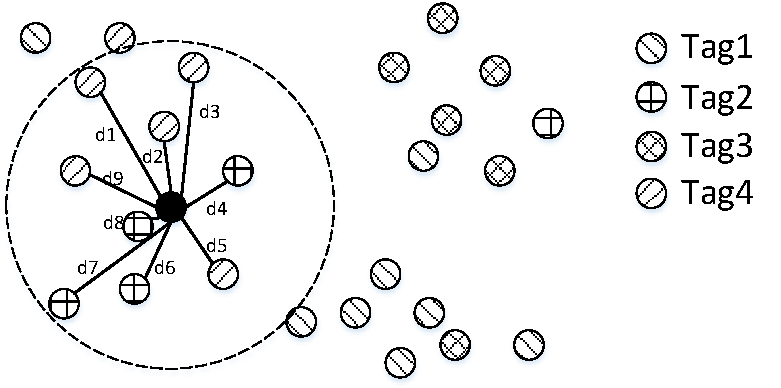
\includegraphics[width=0.4\textwidth]{fig/fig5b.pdf}
}
\caption{The diagram of \emph{KNN} algorithms.}\label{FIG5}
\end{figure}



\begin{figure}[h]%
\centering
\subfigure[In the 1-output setting.]{
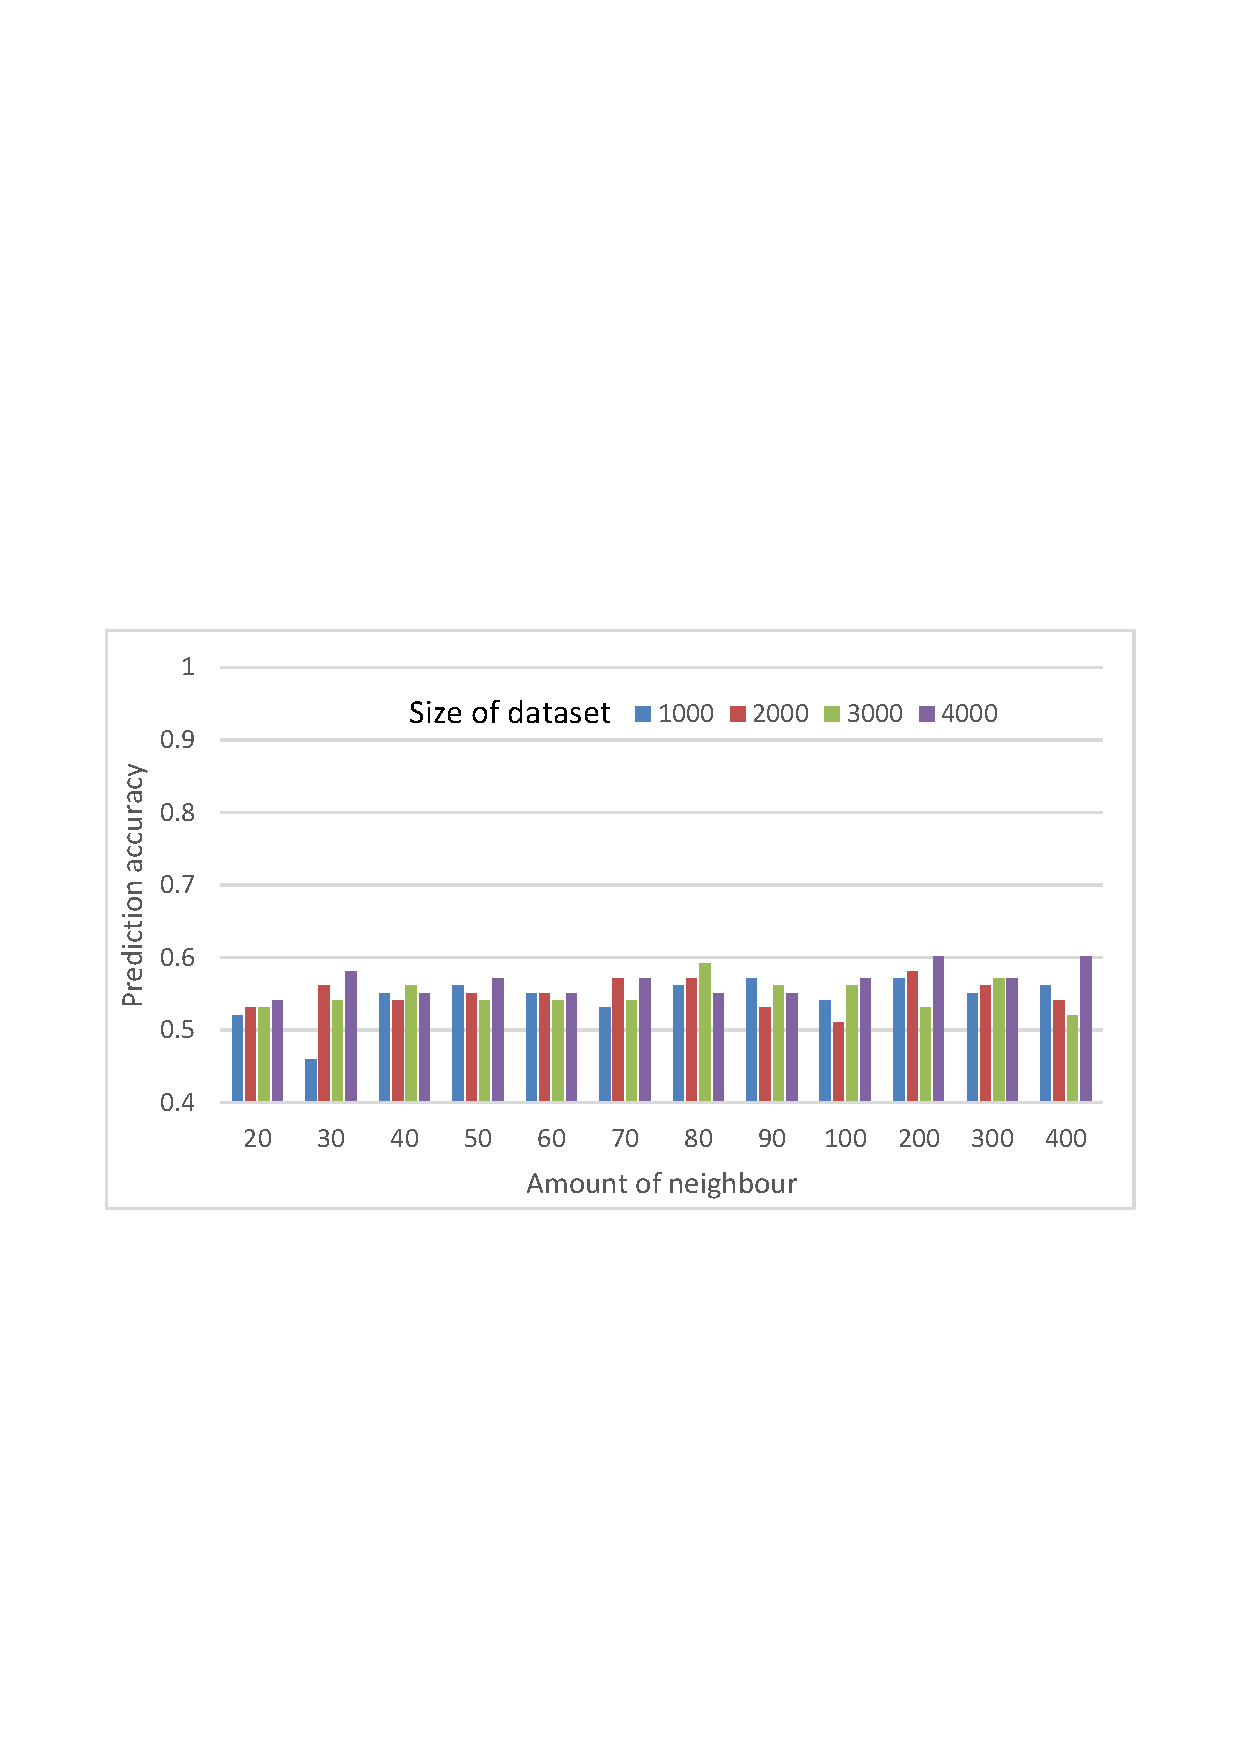
\includegraphics[width=0.4\textwidth,height=2.5cm]{fig/fig7.pdf}
}
\subfigure[In the 10-output setting.]{
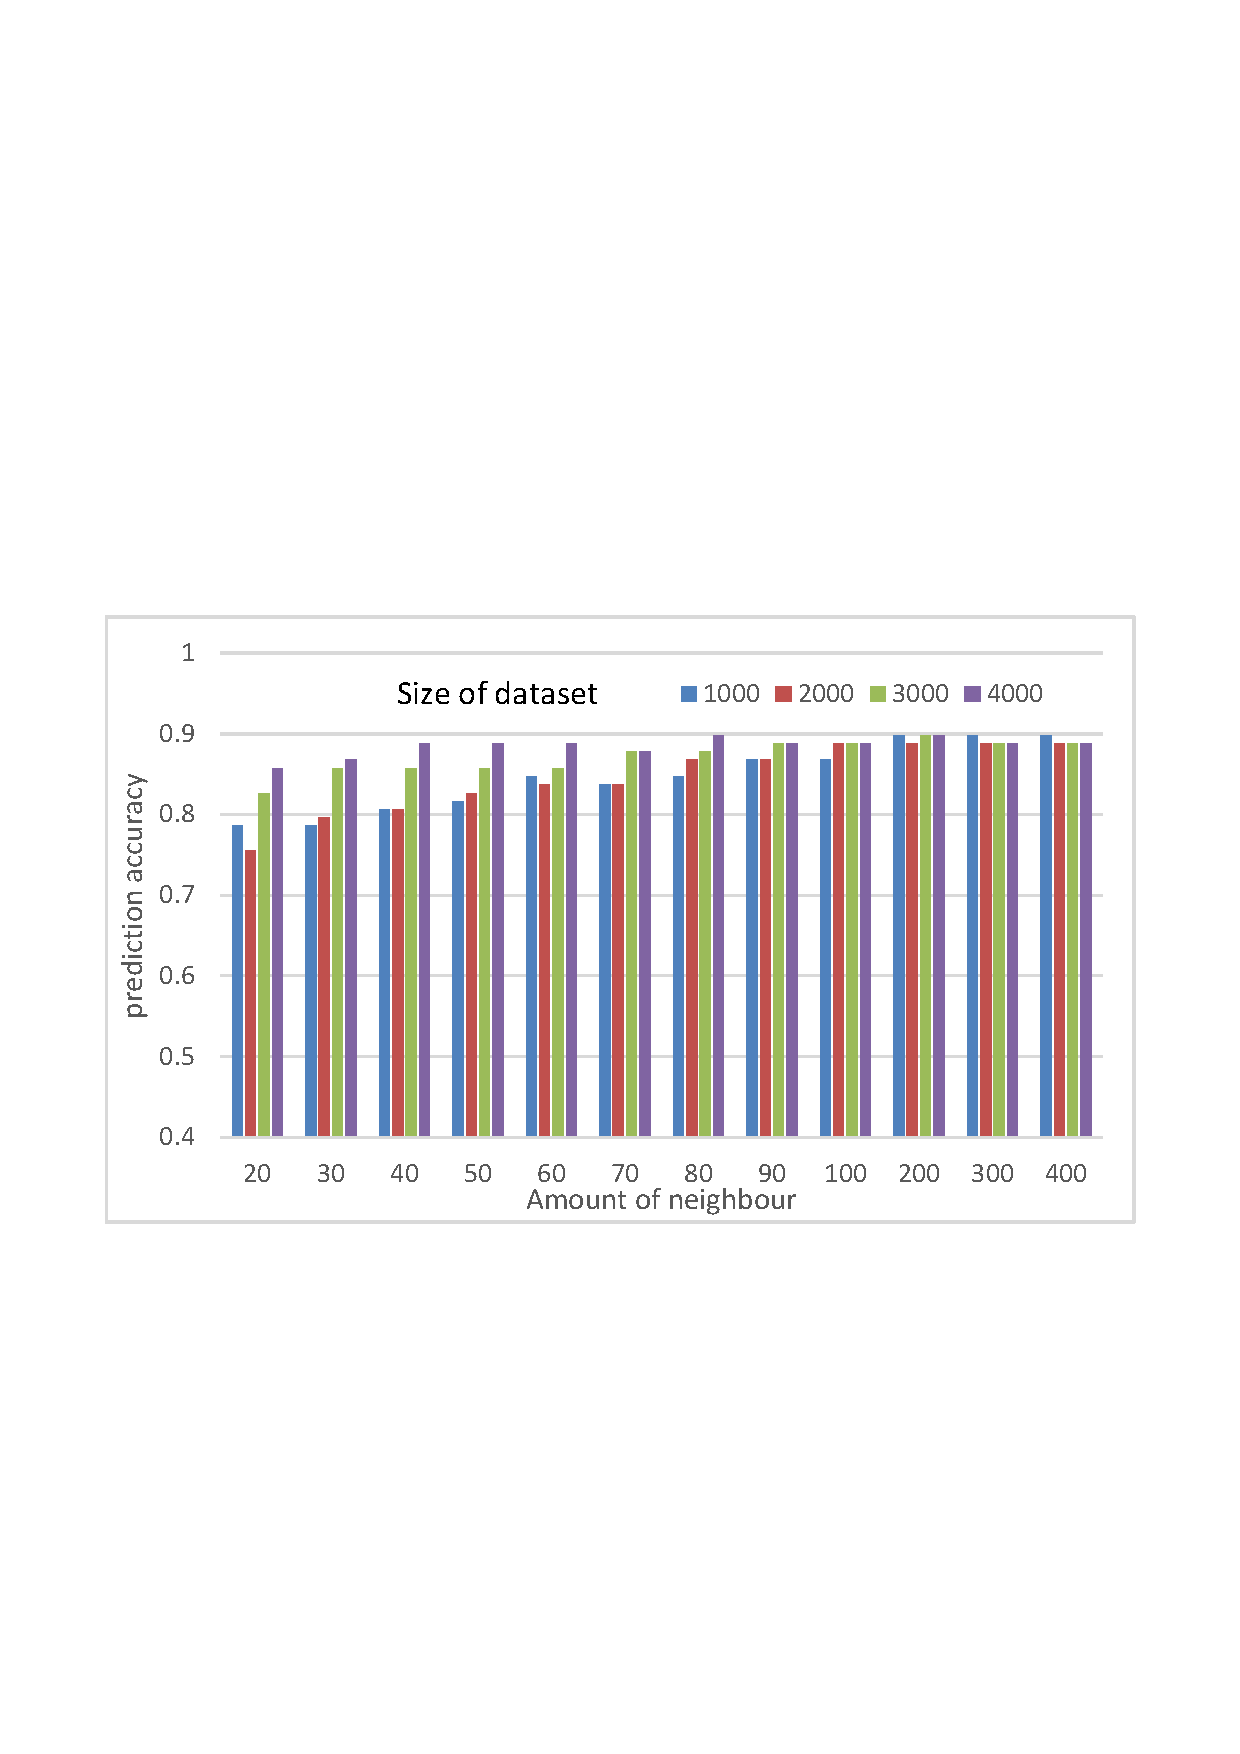
\includegraphics[width=0.4\textwidth,height=2.5cm]{fig/fig9.pdf}
}
\caption{Spectrum of predicting accuracy.}\label{FIG7}
\end{figure}

\begin{figure}[h]%
\centering
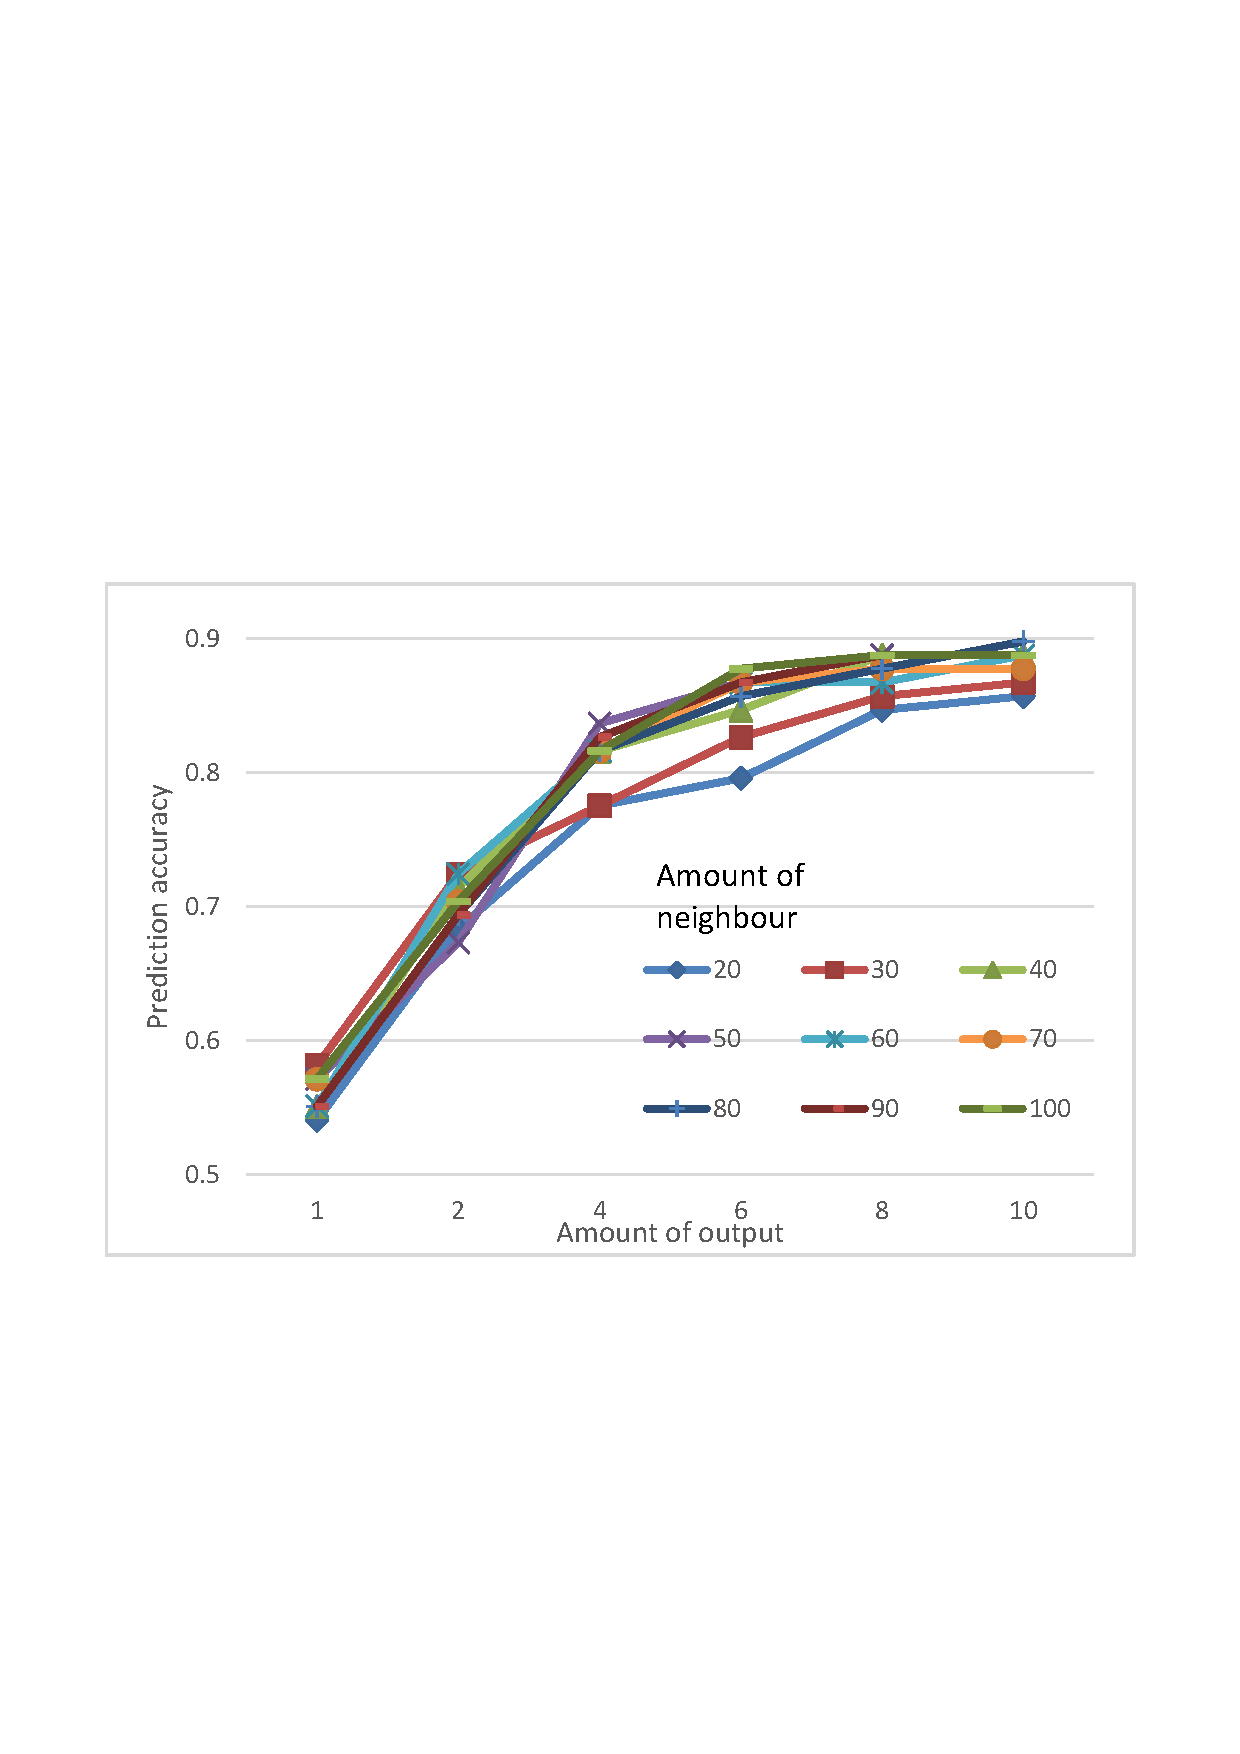
\includegraphics[width=0.5\textwidth,height=3.5cm]{fig/fig8.pdf}
\caption{The relationship between predicting accuracy and the amount of 
output.}\label{FIG8}
\end{figure}

%\begin{figure}[h]%
%\centering
%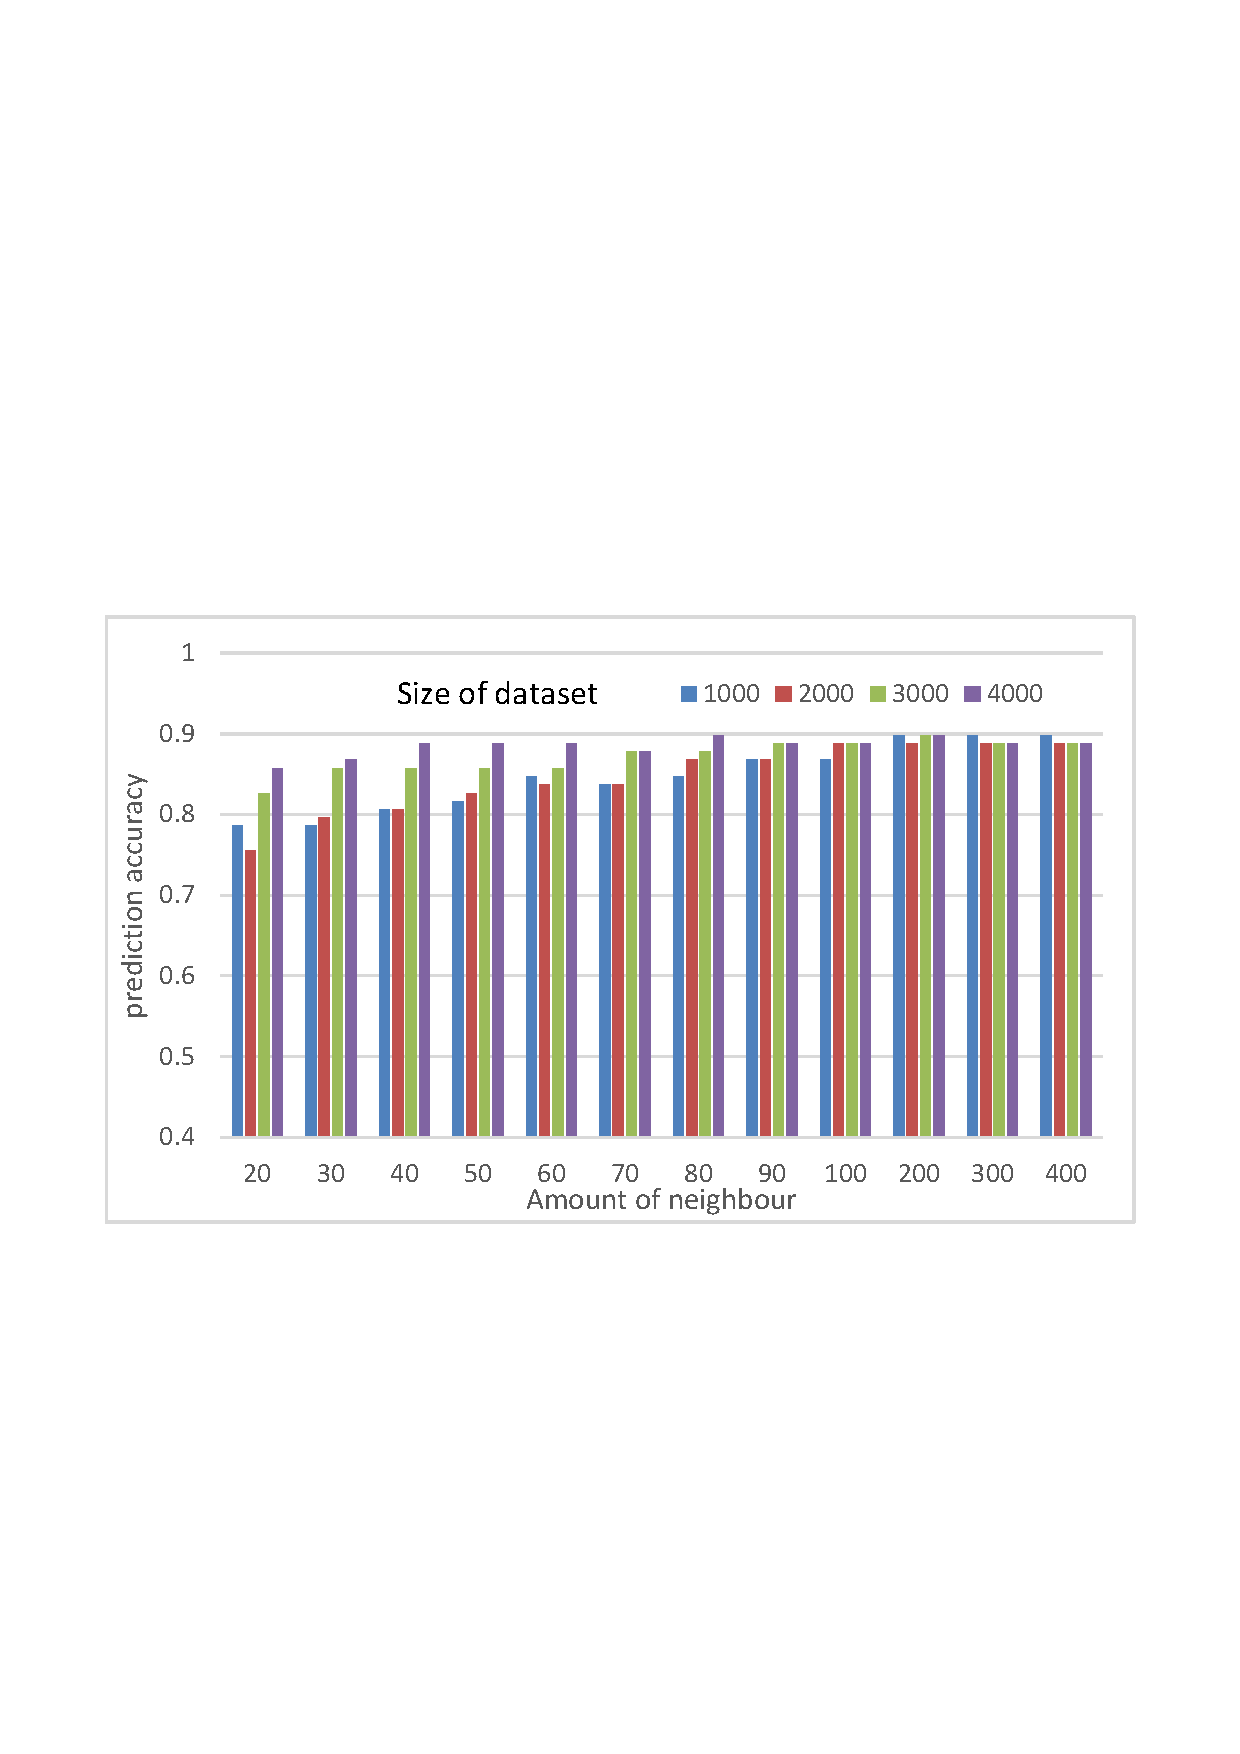
\includegraphics[width=0.5\textwidth]{fig/fig9.pdf}
%\caption{Spectrum of predicting accuracy with 10-output setting.}\label{FIG9}
%\end{figure}

\begin{figure}[h]%
\centering
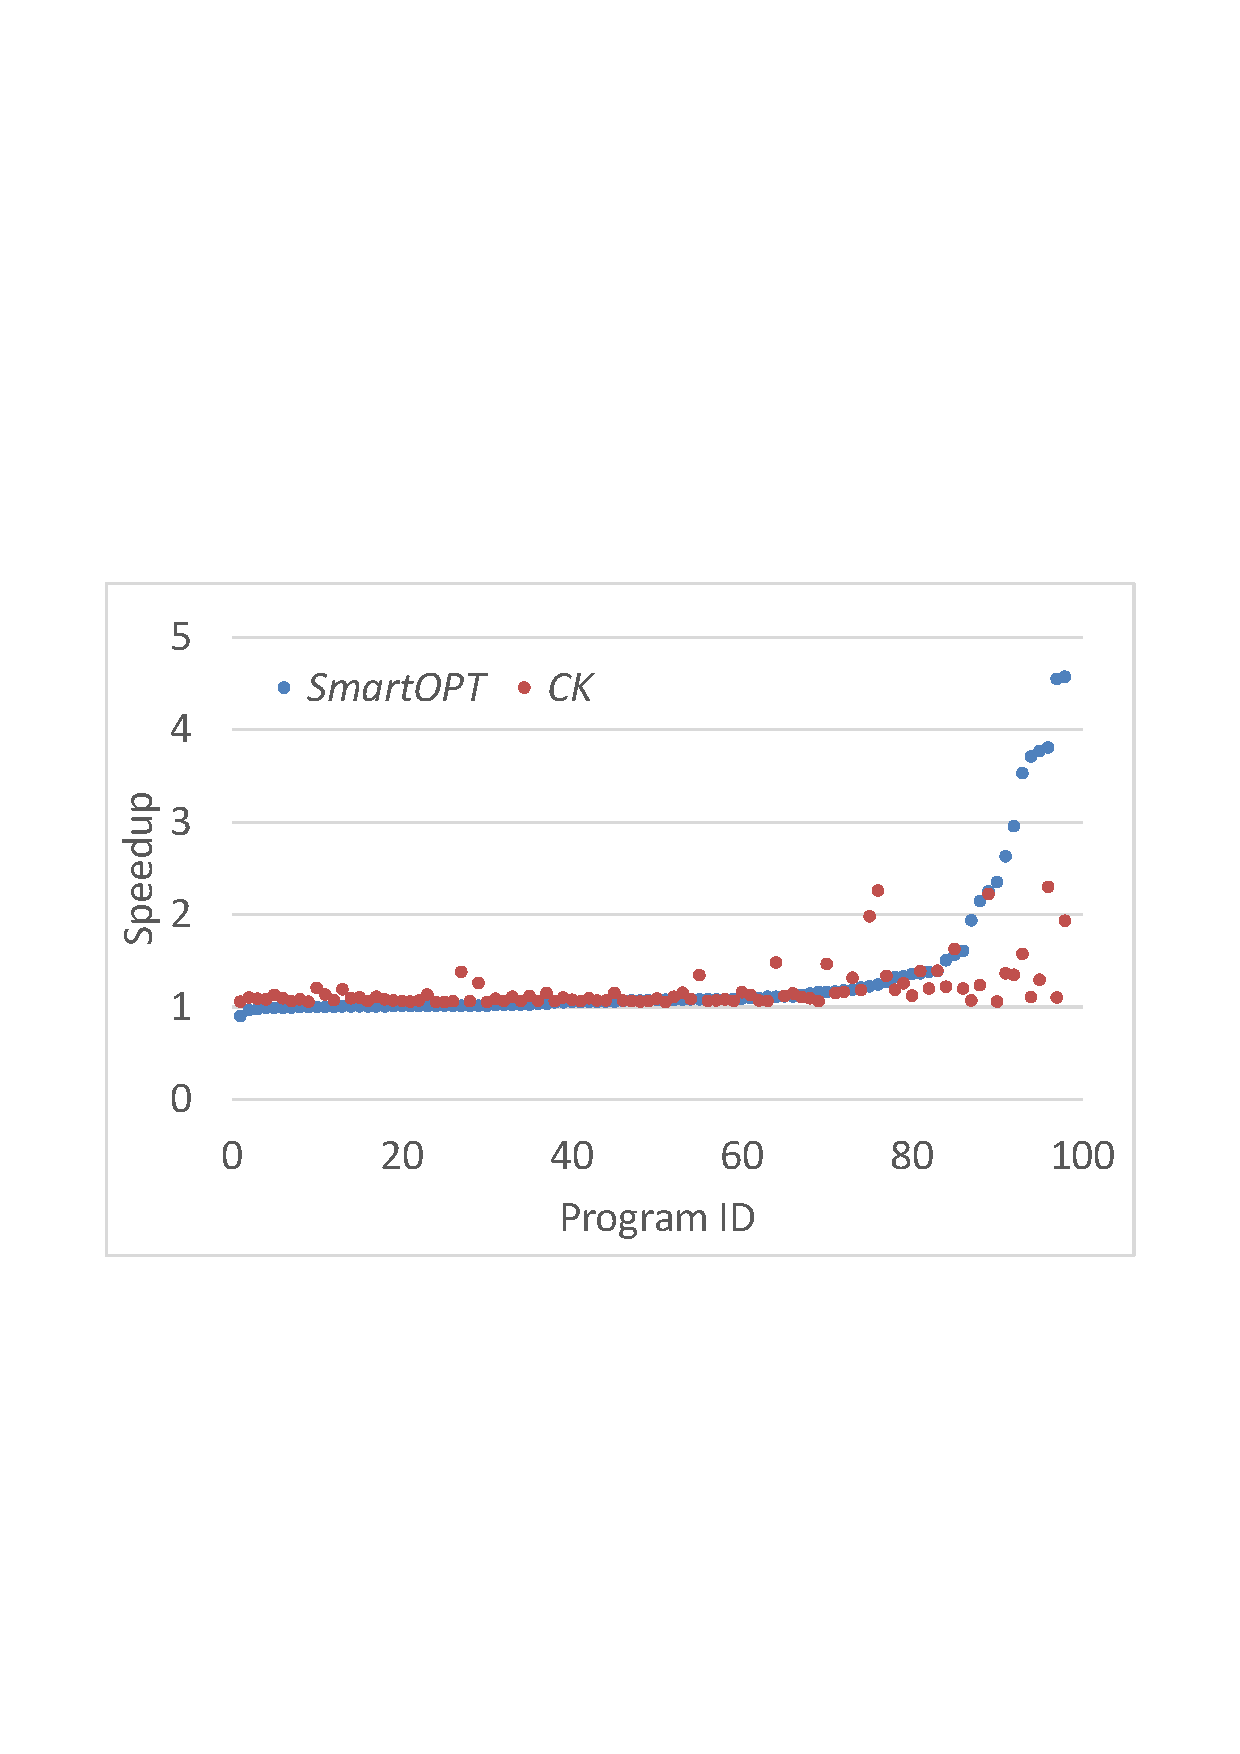
\includegraphics[width=0.5\textwidth,height=3.5cm]{fig/fig10.pdf}
\caption{The speedup comparison of SmartOPT and CK. The metric is illustrated 
in the incremental way.}\label{FIG10}
\end{figure}


\subsection{Comparison between the state-of-art and \emph{SmartOPT}}

In this subsection, we compare \emph{SmartOPT} with the state-of-art. \emph{CK} 
framework is chosen as the baseline. Two metrics are considered, speedup and 
overhead. Speedup means the performance bonus of the programs optimized by 
\emph{SmartOPT} and \emph{CK} individually. And overhead represents the time 
price when programs are handled by each of them.

The baseline of the optimizing level is set as -O2\footnotemark[1]. 
\emph{SmartOPT} is configured with 10 outputs, 4000 dataset and 100 neighbors. 
\emph{CK} is set that each program is iteratively evaluated 30 times. In our 
compiler, there are 184 compiling options in total. In each iteration of 
\emph{CK}, about 10\% options are enabled randomly. So, during all 30 
iterations, the enable probability of each option is 100\%*(1-(1-0.9)30)≈100\%, 
which means the 30 times is enough to cover all compiling options individually. 
100 programs are generated randomly as the micro-benchmarks.

\footnotetext[1]{\emph{SmartOPT} can work based on any optimizing baseline. As 
-O2 is the default setting in the mainstream compiler systems, we consider -O2 
in this subsection for brevity. -O3 case is illustrated in the next 
subsection.}

As \emph{CK} is an iterative based optimizing framework, the overhead of the 
iterative progress is much larger than that of the predicting progress of 
\emph{SmartOPT}. Assuming that the execution time of a program is about 20 
seconds, the 30 times iteration consumes about 20*30=600 seconds. Besides that, 
repetition is necessary in the iterative progress to alleviate the impact of 
the system noise. If we set the repetition time as 4, the iterative progress 
will consume about 600*4=2400 seconds. To make the output more readable, 
\emph{CK} evaluates the options in the yielded group one by one to remove the 
redundant options. This introduces another 10-20 iteration times, which is 
about 10*4*20=800 seconds at least. So, to optimize the compiling options of a 
20-seconds program, \emph{CK} takes 2400+800=3200 seconds, a.k.a. about 1 
hour. Unfortunately, in the engineering field, programs usually take about 
minutes or hours. This exaggerates the drawbacks of \emph{CK}. Our proposed 
\emph{SmartOPT} is built based on the static features of source code. The 
predicting overhead is trivial, which could be claimed less than 10 seconds in 
our experience. On the overhead, \emph{SmartOPT} is superior to \emph{CK}.

Overall, it can be seen that both \emph{SmartOPT} and \emph{CK} have the 
ability to speed up programs with the automatic compiling options adjustment. 
The price \emph{SmartOPT} pays is much less than that \emph{CK} does. It can be 
claimed that \emph{SmartOPT} is more practical than \emph{CK}.

\subsection{Evaluation on \emph{SPEC CPU 2000} \& \emph{SPEC CPU 2006}}

The benchmark suite evaluated in this work is composed of 
\emph{SPEC CPU 2000} \& \emph{SPEC CPU 2006}. The program structure is complex. 
Too many functions are involved. Based on the hot functions yielded by 
profiling, we divided the programs into 131 sub-cases. In each sub-case, a 
single hot function is identified as the target source code. The customized 
compiler system makes instrument for each function automatically to record the 
execution time. \emph{SmartOPT} predicts the compiling options accordingly for 
each of them. The baseline of the optimizing level is set as -O3.

The hot functions are responsible for the main computing progress. They are 
selected according to the following stages.

\begin{enumerate}[1.]
\item The sum of the hottest degree of the functions in a single program is 
	higher than 90\%.
\item Among the functions yielded by the last step, the hot degree of the 
	individual function is higher than 10\%.
\end{enumerate}

Based on the -O3 dataset, \emph{SmartOPT} makes prediction for each sub-cases. 
We compared the performance of the sub-cases with -O3 and those with the 
predicted compiling options. The details are illustrated in Figure~\ref{FIG12} 
and Figure~\ref{FIG13}. As shown in Figure~\ref{FIG12}, 41 out of 71 \emph{SPEC CPU 2000} sub-cases are speeded up, with a maximal performance improvement of 
2.11x. And the average speedup of the 71 sub-cases is about 1.14x. In 
Figure~\ref{FIG13}, 45 out of 60 \emph{SPEC CPU 2006} sub-cases are speeded up. 
4 sub-cases are improved by more than 2x, with a maximal value of 4.99x. The 
average speedup of the 60 sub-cases is 1.25x.

\begin{table}[h]
\begin{center}
\begin{minipage}{\textwidth}
\caption{The compiler options enabled in the \emph{SPEC CPU 2000} and 
	\emph{SPEC CPU 2006} sub-cases (with more than 1.5x speedup).}
	\label{TAB2}%
	\begin{tabular*}{\textwidth}{@{\extracolsep{\fill}}lllp{0.46\textwidth}@{\extracolsep{\fill}}}
\toprule%
Case		     & Sub-case			   & Speedup	& Compiler ptions\\
\midrule
\multirow{2}{*}{164} & compress\_block             & 1.885 	& -fno-cse-follow-jumps -flto -fno-tree-loop-distribute-patterns                         \\
                     & fill\_window                & 1.714 	& -fprefetch-loop-arrays -ftree-loop-if-convert                                          \\
172                  & psinv                       & 1.626 	& -fno-tree-dominator-opts -funsafe-math-optimizations                                   \\
\multirow{2}{*}{186} & EvaluatePawns               & 2.111 	& -flto                                                                                  \\
                     & evaluate                    & 2.099 	& -flto                                                                                  \\
\multirow{2}{*}{462} & quantum\_cnot               & 2.713 	& -fprefetch-loop-arrays -ftree-copy-prop                                                \\
                     & quantum\_toffoli            & 4.992 	& -fprefetch-loop-arrays -funroll-loops                                                  \\
464                  & SetupLargerBlocks           & 2.112 	& -fprefetch-loop-arrays -funroll-loops                                                  \\
481                  & advect\_scalar              & 3.299 	& -ffast-math -fno-guess-branch-probability -fprefetch-loop-arrays                       \\
482                  & vector\_gautbl\_eval\_logs3 & 1.637 	& -fno-modulo-sched-allow-regmoves -fprefetch-loop-arrays -fno-sched-last-insn-heuristic \\
\botrule
\end{tabular*}
\end{minipage}
\end{center}
\end{table}

The compiling options are also analyzed. For the sake of conciseness, only the 
details of the sub-cases with more than 1.5x speedup are revealed in 
Table~\ref{TAB2}. In the 10 listed sub-cases, the most frequently enabled 
options are -fprefetch-loop-arrays (6 times), -flto (3 times), -funroll-loops 
(2 times). The compiler options group {-fprefetch-loop-arrays, -funroll-loops}, 
and {-flto} is enabled twice respectively. It seems that there are some enable 
patterns for compiler options which could speed up certain type of source 
codes. So, we further analyze how many times all 65 compiler options in the 131 
sub-cases are enabled individually. In Figure~\ref{FIG11}. The first 3 
frequently enabled options are -fprefetch-loop-arrays (32 times), -flto (16 
times), -funroll-loops (15 times). And 37 out of 65 options are enabled only 
once. In this work, only brief and simple statements are provided on the 
relations between options and source codes. Due to the complicated interaction 
among compiler options and different types of source code structure, we don’t 
explain why the options should be enabled for the certain source code 
structure.

\begin{figure}[h]%
\centering
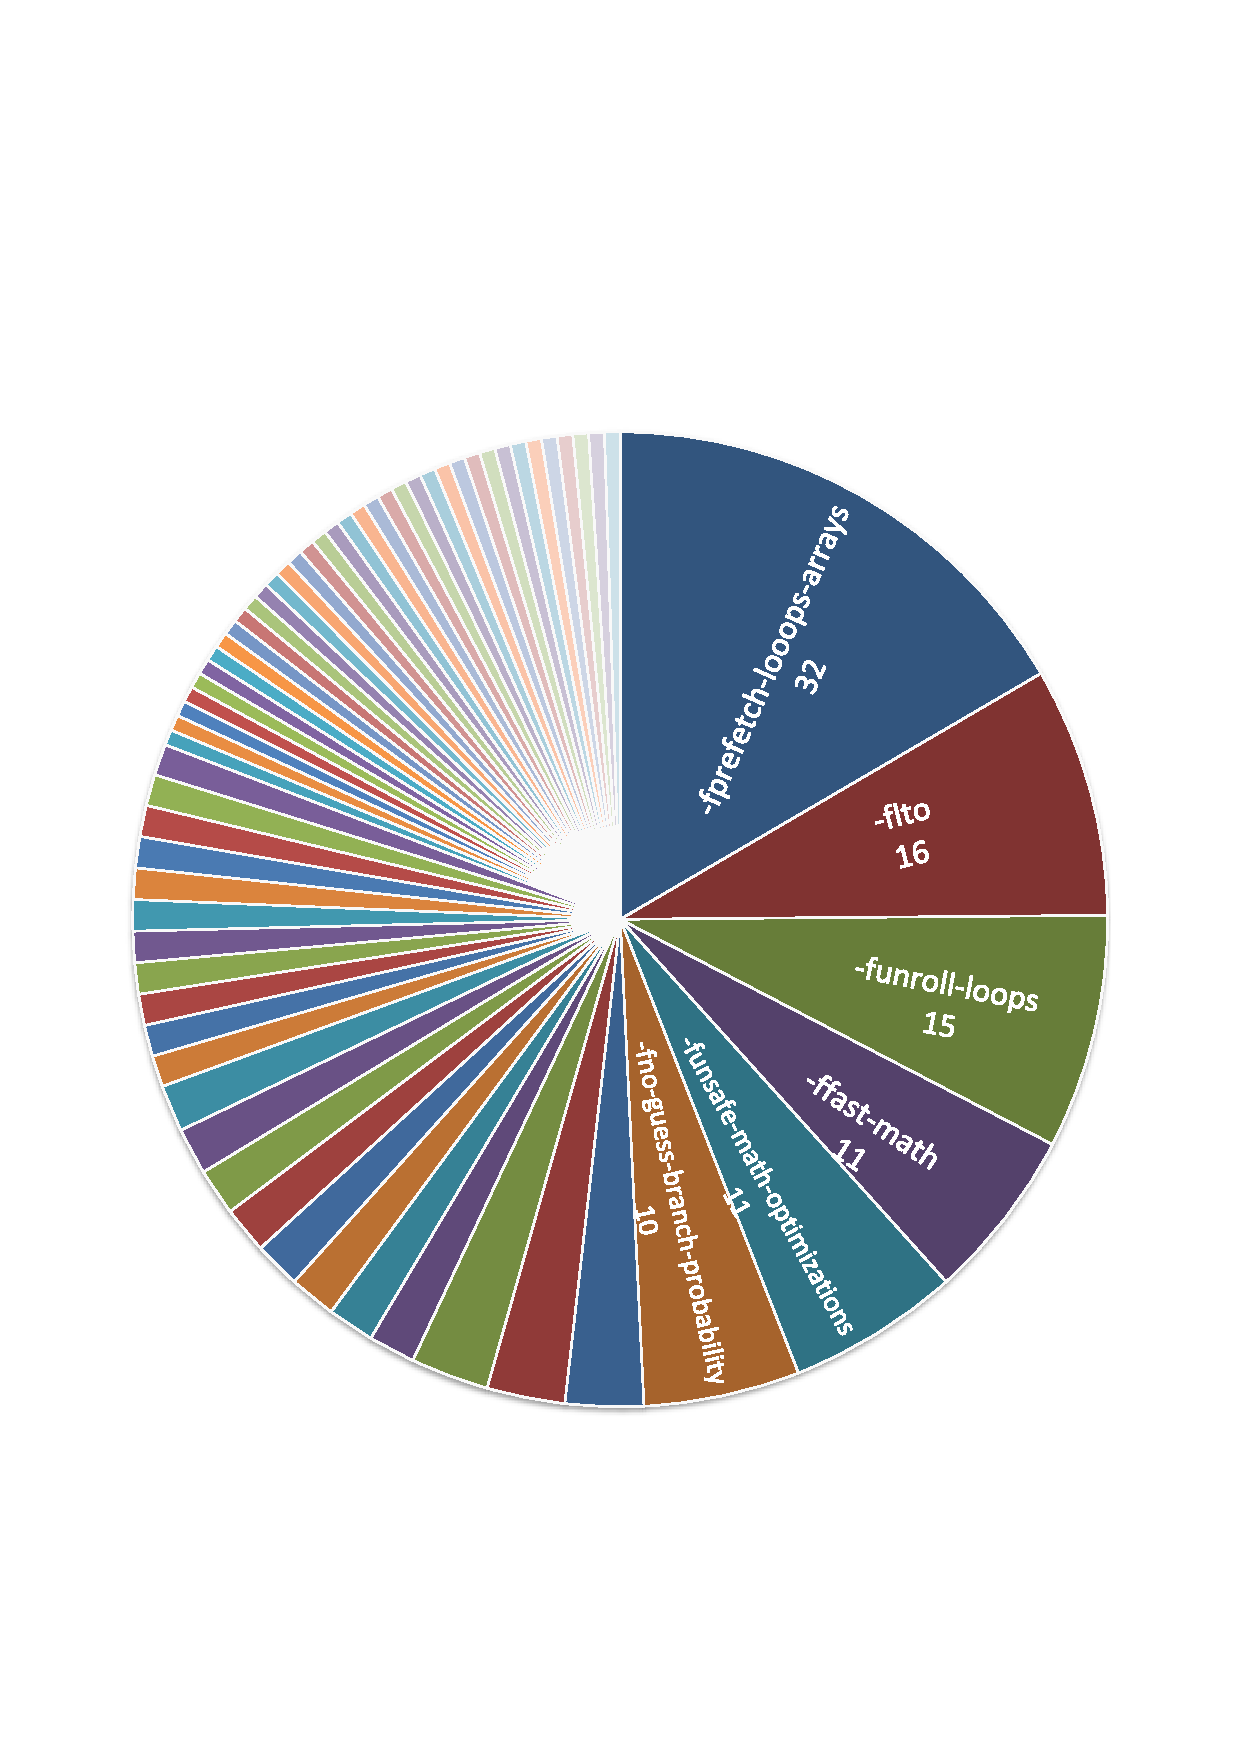
\includegraphics[width=0.4\textwidth]{fig/fig11.pdf}
\caption{The distribution of the 65 compiler options. For brevity, only the 
options enabled more than 10 times are illustrated.}\label{FIG11}
\end{figure}

\begin{figure}[h]%
\centering
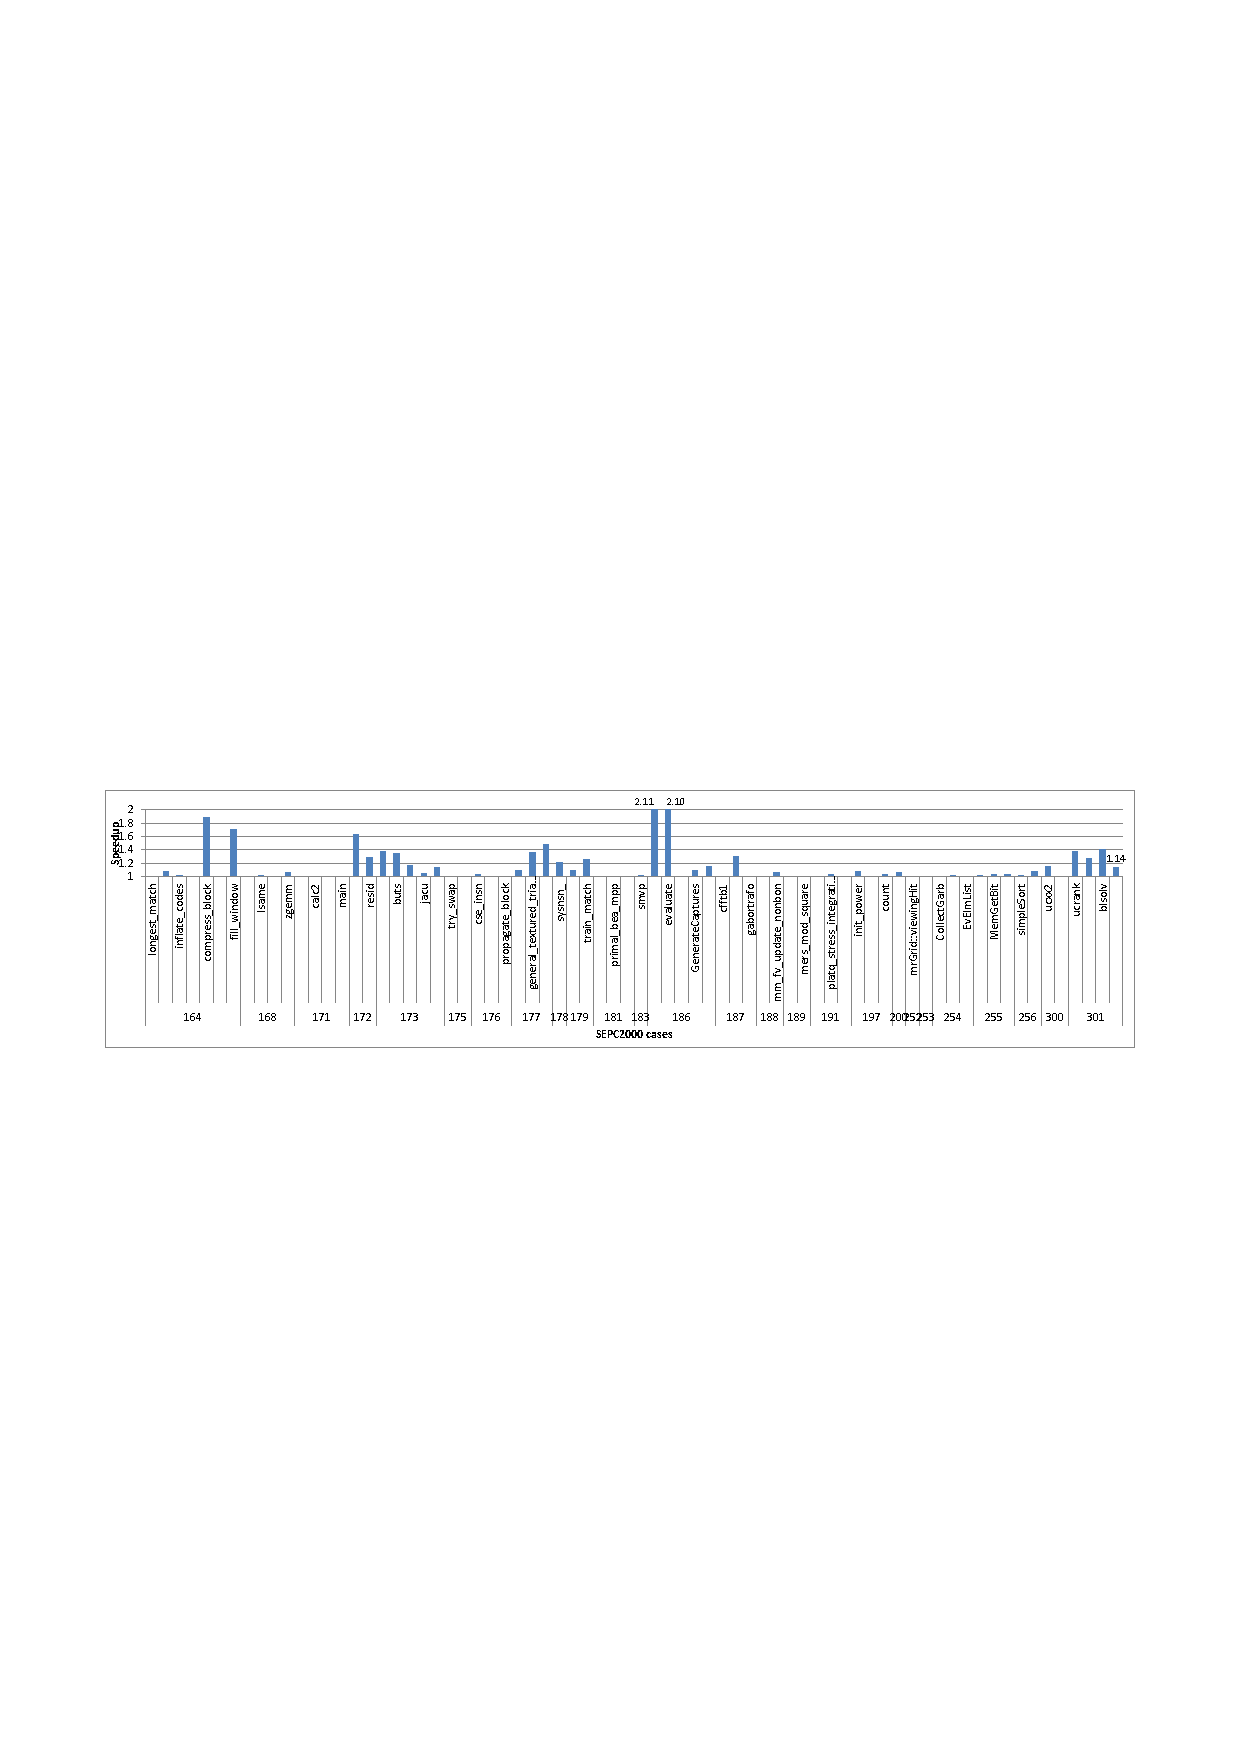
\includegraphics[width=1\textwidth]{fig/spec2000.pdf}
\caption{The speedup of \emph{SPEC CPU 2000} sub-cases. }\label{FIG12}
\end{figure}

\begin{figure}[h]%
\centering
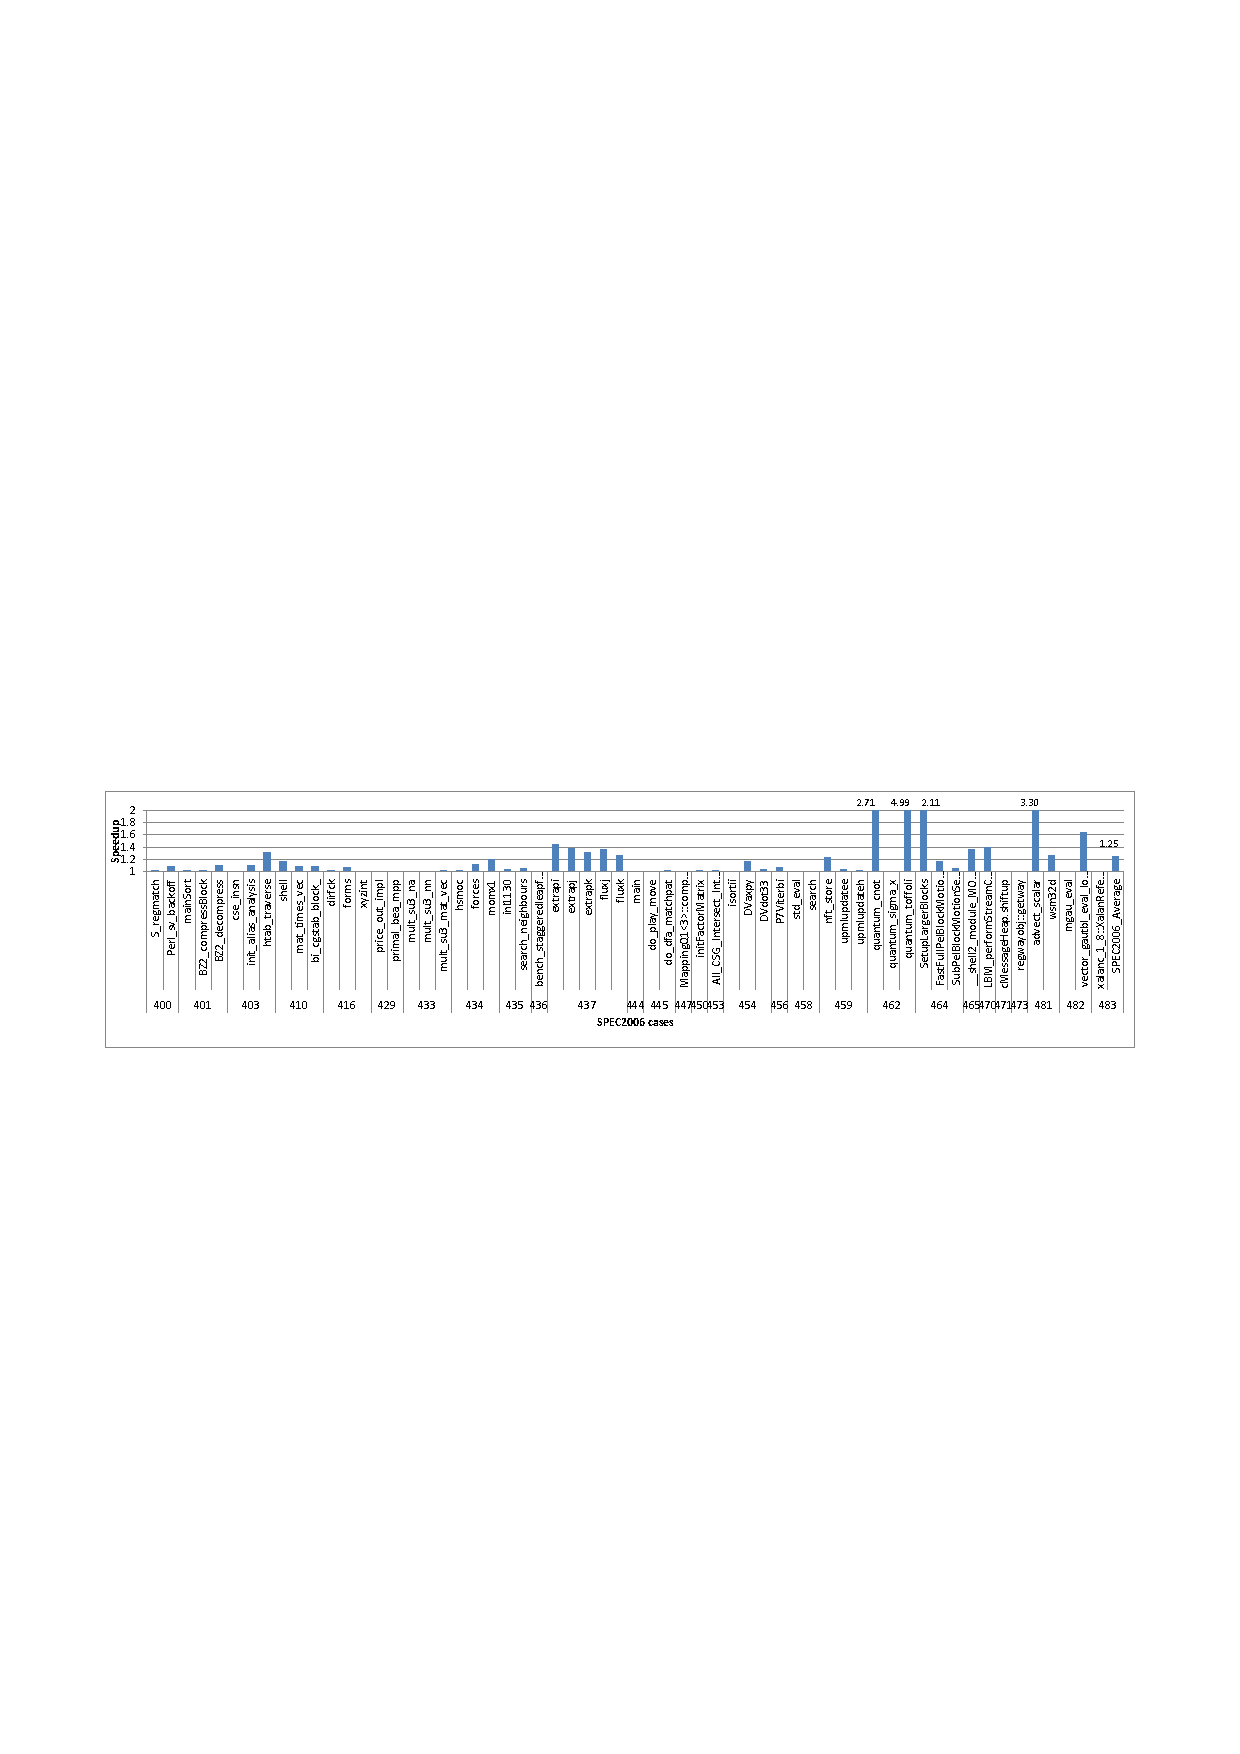
\includegraphics[width=1\textwidth]{fig/spec2006.pdf}
\caption{The speedup of \emph{SPEC CPU 2006} sub-cases.}\label{FIG13}
\end{figure}


\section{Conclusion}\label{sec7}
The modern mainstream compiler relies on the coarse-grained levels to manage 
the compiling optimizing techniques. The fixed optimizing level strategy 
ignores the details of the underlining architecture and the inherence of the 
program. The opportunities for the further performance improvement may be 
omitted. To release power of compiler, we proposed \emph{SmartOPT}, a framework 
which can assist people to make fine-grained optimizing decision. The static 
features of the source code, the rapid construction of dataset and the heuristic 
predicting model make \emph{SmartOPT} superior to the state-of-art. Our proposed 
framework is able to yield the efficient optimizing options with the trivial 
overhead. The systematic evaluation shows the great advantage of 
\emph{SmartOPT}, indicating our framework to be a practicable solution in the 
engineering field.




%%===========================================================================================%%
%% If you are submitting to one of the Nature Portfolio journals, using the eJP submission   %%
%% system, please include the references within the manuscript file itself. You may do this  %%
%% by copying the reference list from your .bbl file, paste it into the main manuscript .tex %%
%% file, and delete the associated \verb+\bibliography+ commands.                            %%
%%===========================================================================================%%

\bibliography{sn-bibliography}% common bib file
%% if required, the content of .bbl file can be included here once bbl is generated
%%\input sn-article.bbl

%% Default %%
%%\input sn-sample-bib.tex%

\end{document}
